\documentclass[a4]{book}
\usepackage{graphicx}
\usepackage{hyperref}
\usepackage{amsmath}
\usepackage{listings}
\usepackage{minted}
\usepackage{natbib}

\bibliographystyle{unsrtnat}

\author{Richard Neher\\Biozentrum, University of Basel}
\title{Physics of Life I}

\graphicspath{{figures/}}

\begin{document}
\maketitle

\chapter*{Preamble}

The laws of physics govern living matter as much as they govern inanimate matter.
However, it is often hard to see how physical principles enter in biology because living matter is constantly in flux, heterogeneous, and never at equilibrium.
Nevertheless, physics can elucidate many seemingly complex phenomena in biology.

In this course -- co-taught with Sebastian Hiller -- we will attempt to how show how biology can not only be described in terms of ``parts lists'' and ``cartoon''-like sketches, but understood in terms of quantitative and predictive relationships.
Such quantitative methods are becoming more and more important in modern biology and require a solid mathematical toolbox and often programming skills.
I encourage you to take a close look again at:
\begin{itemize}
	\item Mathematics: your high-school math and ``Mathematische Methoden I\&II''
	\item Physics: Mechanics, fluid dynamics, and thermodynamics from ``Physics I''
	\item Programming: python note-books and basic programming as you learned in programming and computational courses in the first year.
\end{itemize}

{\bf Lecture notes:}
These lecture notes were first written a few years ago and are adapted to the content of the current course to some extent.
I might make some changes to them over time, add additional materials, or reorder the content.

I am providing these lecture notes for your convenience.
Even though they look polished (typeset with LaTex), they are just notes.
There will be typos, errors, and incomplete sections.
I hope to develop them over the years to come and encourage you to read them with a critical eye.
Be critical, report potential errors, and give feed-back on form and content.

\section*{Suggested reading}
There is no one book covers the material planned for this course.
But the following books touch on the subject and are recommended:
\begin{itemize}
	\item \href{https://www.google.com/url?sa=t&rct=j&q=&esrc=s&source=web&cd=1&cad=rja&uact=8&ved=2ahUKEwjd4-XS6tfkAhVI2qQKHSBoDFUQFjAAegQIAhAB&url=https%3A%2F%2Fwww.crcpress.com%2FPhysical-Biology-of-the-Cell%2FPhillips-Kondev-Theriot-Garcia%2Fp%2Fbook%2F9780815344506&usg=AOvVaw1S0mgI830cAwjb4G48vKPF}{\bf Physical Biology of the Cell} by Hernan Garcia, Jane Kondev, Julie Theriot, and Rob Phillips.
	\item \href{http://book.bionumbers.org/}{\bf Cell Biology by the Numbers} by Rob Phillips and Ron Milo.
	\item \href{https://press.princeton.edu/titles/112.html}{\bf Random Walks in Biology} by Howard Berg
\end{itemize}

% scales
 %!TEX root = main.tex
\chapter{The relevant scales: sizes, energies, concentrations}

\section{Units and dimensions}
Objects and events in the world around us have quantifiable properties such was length, mass, duration, charge, etc.
These nature of these properties are often called dimensions and for each of these dimensions, we have one or several units in which we measure them: grams, meters, seconds etc.
Fundamentally, all these measurements are comparisons between quantities of the same dimension.
We measure the length of an object by comparing it to a stick of a particular length -- one meter.
These units have been agreed upon and are usually chosen to be convenient for a particular use case.
A meter, for example, is roughly one step.
Importantly, we can only compare things of the same dimension: length with length, mass with mass, etc.
There no sense in which you can meaningfully compare a quantities of different dimensions, for example one measured in meters to another one measured in kilograms.

Physical laws, on the other hand, relate quantities of different dimensions to each other.
Take Newton's law:
\begin{equation}
	F = m\times a \quad\quad \mathrm{Force [N]} = \mathrm{mass [kg]}\times \mathrm{acceleration [m/s^2]}
\end{equation}
The unit of force (Newton) is a product of the units of mass (kilogram) and acceleration, which itself as dimension length/time$^2$ and is measured in meter/second$^2$.

Whenever you specify a physical quantity, you have specify the unit!

\section{The relevant scales}
To quantitatively understand how different biological processes and phenomena relate to each other, it is essential to get a sense of the relevant length, force, energy, and concentration scales.
A very useful collection of important quantities is available at \href{http://book.bionumbers.org}{bionumbers.org} by Ron Milo and colleagues.
Once we have identified the relevant scales and sizes, simple reasoning and comparing different scales can already give us quite robust insight into many cell biological properties.

\subsection{How small are things?}
The following table has (very) rough numbers for the different sizes involved

\begin{itemize}
  \item $3\times 10^{-10}$m (0.3nm): height of one DNA base pair
  \item $2\times 10^{-9}$m (2nm): diameter of DNA, typical protein diameter
  \item $2\times 10^{-8}$m (20nm): bacteria phage
  \item $10^{-7}$m (0.1$\mu$m): animal virus
  \item $10^{-6}$m (1$\mu$m): bacterial cell
  \item $2\times 10^{-6}$m (2$\mu$m): yeast cell nuclei
  \item $10^{-5}$m (10$\mu$m): eukaryotic cell
\end{itemize}

\begin{figure}[h]
	\centering
	\includegraphics[width=\textwidth]{100-f1-LengthScalesGraphic-14.png}
	\caption{The range of linear dimensions relevant in a cell from \href{http://book.bionumbers.org/size-and-geometry-introduction/}{book.bionumbers.org}}
	\label{fig:length_scales}
\end{figure}

With this huge range of linear dimensions, volume and mass vary over a much larger range still.
It is useful to remember: One liter is $10^{-3}m^3$, one milliliter is a $cm^3$ (the size of an eppendorf tube), one femto liter is $\mu m^3$. One gram of water is roughly one milliliter.
Using the length scales above, we get the following rough volume scales for biological entities (there is obviously a lot of variation between cell and virus types).

\begin{itemize}
  \item $10^{-20}$l: volume of a bacteria phage
  \item $10^{-15}$l (1fl): volume of a bacterial cell
  \item $10^{-12}$g (1pg): weight of a bacterial cell
  \item $10^{-12}$l (1pl): volume of a eukaryotic cell
\end{itemize}

Humans weigh roughly 100kg (100l volume) and most of ``human stuff'' is made from cells. Given the rough weight of a cell, we estimate $10^{14}$ human cells in the human body.
The true number is closer to $10^{13}$, but this discrepancy is within the accuracy of our calculation.
Furthermore, we immediately see that a comparable number of bacterial cells will contribute rather little to the total weight since the individual cell is 1000-fold lighter.


\subsection{Typical genome sizes}
Genome sizes vary enormously among species.

\begin{itemize}
  \item $3\times 10^{2}$bp: viriods (one tweet)
  \item $10^{4}$bp: typical RNA viruses (one page)
  \item $10^{5}$bp: animal DNA viruses (10 pages)
  \item $10^{6}-10^{7}$bp: bacterial genome (a serious book)
  \item $3\times 10^{9}$bp: human genome (one tenth of all of English wikipedia)
\end{itemize}

Genome size among animals and plants correlates little with perceived complexity of the organism.


\begin{figure}[h]
	\centering
	\includegraphics[width=\textwidth]{502-f1-GenomeSizesRanges-1.png}
	\caption{Illustration of the range of genome sizes from \href{http://book.bionumbers.org/size-and-geometry-introduction/}{book.bionumbers.org}}
	\label{fig:genome_sizes}
\end{figure}

It is instructive to compare cell dimensions versus the length of the DNA molecule that needs to fit inside:
\begin{itemize}
  \item $10^{-6}$m (1um): length of a phage genome.
  \item $10^{-3}$m (1mm): length of the bacterial genome ($3\times 10^9$ bases a 0.3nm each)
  \item $1$m (1m): length of the human genome ($3\times 10^9$ bases a 0.3nm each)
\end{itemize}

We see that DNA is much longer than the containing cells, see Fig.~\ref{fig:DNA_packing_illustration}.
An amusing little calculation: if DNA from all $10^{13}$ cells of a human body was strung together, it would cover the distance to the sun ($1.5\times 10^{11}$m) more than 100 fold (accounting for the diploid nature).

\begin{figure}[tb]
	\centering
	\includegraphics[width=0.6\textwidth]{bacterial_genome}
	\includegraphics[width=0.25\textwidth]{lysed_ecoli}
	\caption{Left: a typical cartoon suggesting the length of a bacterial chromosome is similar to the length of the cell. Image source: \href{https://www.kissclipart.com/bacterial-genome-clipart-plasmid-genome-bacteria-dt3adi/}{kissclipart}.
	Right: The DNA from an actual E.~coli cell that was lysed (the blob in the middle). A bacterial chromosome of length $5\times 10^6$bps is about 1.5mm long -- roughly 1000-fold the length of the cell.  Clearly, the DNA has to be pretty tightly packed inside the cell. Image source: \href{https://www.nature.com/scitable/content/supercoiled-chromosome-of-e-coli-44517/}{R. Kavanoff}}
	\label{fig:DNA_packing_illustration}
\end{figure}


\subsection{Forces and energies}
So far, we have looked at dimensions and the objects involved could have been dead or alive.
Lets now turn to the energies, power, and forces.
From our daily life, we are used to power on the scale of 100W. This would be your standard (old fashioned) light bulb or the typical power consumption of the human body.
Energy is stored in batteries, reservoirs, or petrol.
In cells, the energy currencies are very different.
The ultimate source of energy (free energy, really) is the sun.
It emits black body radiation at a temperature of 5800K which corresponds to an emission maximum at a wavelength of 550nm in the visible range.
A single photon with wavelength $ \lambda = 500nm$ has the following energy:
\begin{equation}
E = \frac{hc}{\lambda}\approx \frac{1.24 eV\mu m}{\lambda}\approx 2.5eV
\end{equation}
Electron volt (eV) is a unit of energy commonly used in physics. One eV corresponds to the energy required to move one election one Volt up in an electric potential.
Chemists like to measure energy per molecule or reaction and typically use units like $kJ/mol$ or $kcal/mol$.
In a biological system, different energy units are often more convenient.
The most important energy scales in biological systems are the thermal energy kT and the energy released when hydrolyzing ATP to ADP.
The scale kT is important since process that operate on the scale of kT or below happen spontaneously and reversibly, that is they are strongly affected by the randomness to thermal noise.
Controlled and precise reactions typically involve energy differences larger than kT.
Hence it is always important consider an energy difference in relation to kT
\begin{equation}
	kT \approx 0.025eV \approx 0.6 kcal/mol \approx 2.5 kJ/mol \approx 4pN \times nm
\end{equation}
One visible photon is therefore about 100kT, much more than the thermal energy scale.
It is thus plausible that individual visible photons can drive biological processes such as trigger signaling cascades.
To fix one $CO_2$ molecule, around 8 such photons are needed.

The dominant energy currency of the cell is ATP which is hydrolyzed to ADP to power other reactions
\begin{equation}
ATP + H_2O \rightarrow ADP + P_i \quad -30 kJ/mol \approx -12kT
\end{equation}
Again, one ATP hydrolysis is above the thermal energy scale, but not all that far away.
In practice, the (free) energy released in ATP hydrolysis can vary by a factor of two depending on Mg${}^{2+}$ concentration and the concentrations of ATP and ADP.

\begin{figure}[t]
	\centering
	\includegraphics[width=\textwidth]{300-f1-EnergyAxis-11.png}
	\caption{Illustration of the range energy scales from \href{http://book.bionumbers.org/size-and-geometry-introduction/}{book.bionumbers.org}}
	\label{fig:genome_sizes}
\end{figure}


\subsection{Concentrations and molecule counts}
Concentrations are statements about the number of molecules per volume.
There are typically measured as moles per liter, that is $6\times 10^{23}$ molecules per $10^{-3}m^{3}$.
For our purposes, it is useful to express this as number of molecules per femtoliter or $\mu m^3$: 1M=$6\times 10^{23}/10^{15}\mu m^3 = 6\times 10^{8}/\mu m^3$
Hence one nM corresponds to roughly one molecule per bacterium, pM to one molecule per eukaryotic cell.
If proteins are only present in small numbers inside cells or organelles, their individual behavior and the associated stochasticity can be very important.
When thinking about rare molecules, for example signaling molecules, numbers are a better guide than concentrations.

\begin{figure}[h]
	\centering
	\includegraphics[width=\textwidth]{200-f1-ConcentrationAxis-11.png}
	\caption{Illustration of the range concentrations from \href{http://book.bionumbers.org/size-and-geometry-introduction/}{book.bionumbers.org}}
	\label{fig:genome_sizes}
\end{figure}

% \subsubsection{Stochasticity of molecule numbers}
% Fluctuations are important, when molecules are rare.
% But how much do we expect molecule number to fluctuate?
% Consider a simple process where molecules are added at random times with rate $b$ and decay with rate $d$.
% \begin{equation}
% \begin{split}
% 	n &\rightarrow n+1 \quad \mathrm{with\ rate}\ b \\
% 	n &\rightarrow n-1 \quad \mathrm{with\ rate}\ nd
% \end{split}
% \end{equation}
% There are two things to note here:
% (i) Rates have units of 1/time. In a short time interval $dt$ we expect on average $b\ dt$ new molecules to be produced.
% (ii) The production rate is independent of $n$, while the decay rate increases with $n$ since each particle can decay on its own.
% Intuitively, one expects a balance between production and decay such that the number of molecules settles at a value where these two rates match
% \begin{equation}
% 	b = d \bar{n} \quad \Rightarrow \bar{n} = \frac{b}{d}
% \end{equation}
% This results makes sense: $\bar{n}$ increases with increasing production and decreases with increasing decay rate.
% It happens to be the correct expression for the average number of particles $\bar{n}$.
% When $\bar{n}$ is small, however, the actual number of particles will fluctuate a lot around the average value.
% Such stochasticity is captured by a probability distribution $p(n)$.
% At steady state, we the rates between $n$ and $n+1$ need to balance each other.
% \begin{equation}
% 	p(n-1) b = dn p(n) \quad \Rightarrow \quad p(n) = \frac{b}{dn}p(n-1)
% \end{equation}
% This condition has a simple solution:
% \begin{equation}
% 	p(n) = \frac{(b/d)^n}{n!}e^{-b/d}
% \end{equation}
% This distribution is known as the Poisson distribution, where $n!=n(n-1)(n-2)\ldots 1$ is the factorial.
% It has mean $\bar{n} = b/d$ and variance $\sigma^2 = \bar{n}$ (verification is left as exercise).
% The fact that the variance equals the mean is extremely important.
% The variance is the average squared deviation from the mean.
% The typical deviation from the mean is therefore the square root of the variance.
% This relationship -- noise increasing with the square root of the signal -- is very general and underlies most statistical analysis methods.

\subsubsection{Concentrations, energy, and entropy}
Like temperature, concentrations tend to homogenize spontaneously: connect two reservoirs with different concentrations and over time the two concentrations will tend towards the average concentration through diffusion of molecules.
This homogeneous state is the state of highest entropy.
We will see later in the course that the mathematics describing the dynamics of concentrations is very similar to that of concentrations.

A central (and often unintuitive) aspect of thermodynamics is the interplay of \emph{Energy} and \emph{Entropy}.
Concentration gradients represent a state of low entropy.
Such concentration differences are ubiquitously exploited in biology to drive processes like nuclear transport, ATP synthesis, or neuronal signaling.
This effect is most obvious when considering solutions of positively and negatively charged ions on two sides of a membrane that is only permeable to ions of one charge (for example protons) and not the other charge.
Now assume that initially on each side of the membrane positively and negatively charged ions are present in equal concentrations and thus balance each other.
If the concentration $c_{left}$ is high on one side and low $c_{right}$ on the other side, the type of ion that can cross the membrane will start flowing from left to right.
With this flux, a potential difference builds up that opposes further ion flux until the ion flux stops.
How high is the final potential difference $\Delta V$ where the entropy gain due to mixing is balanced by the potential difference between the reservoirs?

This can be estimated using results from statistical mechanics.
The energy difference of an ion with charge $l$ in the left and right reservoir will be $l\Delta V$.
The probabilities of observing it on the left or right in equilibrium (assuming everything else is equal) are therefore related by $p_{left}/p_{right} = e^{-l\Delta V/kT}$.
This ratio, however, is exactly the ratio of the equilibrium probabilities (not that the flux of ions is typically so small compared to the overall concentrations that we can treat the latter as constant).
\begin{equation}
	\frac{c_{left}}{c_{right}} = \frac{p_{left}}{p_{right}} = e^{-\frac{l\Delta V}{kT}} \quad \Rightarrow \quad kT \log(c_{left}/c_{right})  = - l\Delta V
\end{equation}
We see that the potential difference is proportional to the logarithm of the concentration difference!
This is the famous Nernst potential.
It directly connects the thermal energy scale $kT$, the entropy (logarithmic concentrations), and the potential energy.

A pH difference of 1 (ten fold difference in $H^+$ ion concentration) then corresponds to a potential difference of
$\log(10) \approx 2.3 kT \approx 0.06 eV$ or $60meV$.
Typical potential differences across membranes are of the order of $100meV$.

\section{Estimating orders of magnitude}

\subsection{Molecular motors}
Cells have molecular motors that they use to move things around, drive cilia and flagella, or open up the DNA double strand.
Most of these hydrolyze ATP, one molecule at a time.
Some of these motors (kinesin and dynein) move in steps along filaments.
These steps are on the order of 10nm.
Assuming the energy of one ATP hydrolysis is converted with 100\% efficiency into mechanical energy, we expect a maximum force (stall force) of

\begin{equation}
\frac{12kT}{10nm} \approx \frac{48pN nM}{10nm} \approx 5pN
\end{equation}

This estimate is surprisingly accurate -- most ``walking'' molecular motors have \href{http://bionumbers.hms.harvard.edu/bionumber.aspx?&id=112209&ver=1&trm=stall%20force}{stall forces in this range}.


\subsection{Genome replication}
If a genome has a single origin of replication, the rate of genome replication $\kappa$, genome size $L$, and division time $\tau$ are naively related by

\begin{equation}
\kappa = \frac{L}{\tau} = \frac{5\times 10^{6}}{2500s} \approx 2\times 10^3/s
\end{equation}
where we have used a typical bacterial genome size of 5Mb and a division time of 40min.
2000 bases per second is not far off, but probably a factor of 5 too high.
Furthermore, E.~coli can divide in 20min rather than 40min.
The discrepancy can resolved by observing that (i) replication proceeds via two replication forks, and (ii) the next replication is started before the first one is complete.

Eukaryotic replication machinery is no faster than the prokaryotic ones, but the genomes are 1000 fold larger.
To replicate their genomes in reasonable time eukaryotic genomes have 1000s of origins of replication.

\subsection{Take home messages}

\begin{itemize}
    \item For quantitative reasoning, it is important to have a sense of the relevant scales!
    \item Simple ``back-of-the-envelope" calculation can give you important insights into the nature of a problem
    \item Many processes in biology happen at low copy numbers and with energies close to $kT$. Stochastic effects are important.
\end{itemize}

\section{Differential equations}
Mathematics, and differential equations in particular, are the language suitable to describe, analyze, and predict quantitative phenomena.
Some knowledge of differential equations is essential, and this should have been covered in high school and last year's courses.

There are many excellent treatise of differential equations out there.
We will review this topic and discuss how such equations are solved numerically in the lecture.



% \subsection{The number of ribosomes}
% In an exponentially growing bacterial culture, biomass doubles once every division time.
% About one fourth of the cell mass is protein, which comes down to
% \begin{equation}
% N_{aa} = 0.25 \times 10^{-12} g/cell \times 6\times 10^{23} \frac{Da}{g} / 100 \frac{aa}{Da} \approx 10^9 aa/cell
% \end{equation}
% amino acids per cell that need to be synthesized every 20min and incorporated in to peptides.
% Peptide synthesis rate of 10aa/s, a single ribosome can process about $10^4$ amino acids per cell cycle, suggesting the cell needs at about $10^5$ ribosomes.
% This is roughly what is measured. Again, \href{http://book.bionumbers.org/how-many-ribosomes-are-in-a-cell/}{bionumbers.org} has a very nice description of this problem.
% Importantly, this quick calculation tells us that ribosomes make up a substantial fraction of the total cell proteome (they certainly dominate the RNA pool).



 %!TEX root = main.tex
\chapter{Differential equations in physics and biology}

Most laws of physics and mathematical models of biology are formulated as differential equations.
While these descriptions are often abstract and solving them can be complicated, differential equations are a very natural and intuitive way of describing the world.
The type of differential equations we will consider describe how the state of a system changes over time.

Fig.~\ref{fig:ode} shows two simple settings that can readily described by ordinary differential equations (ODEs).
In the first case, we consider a bucket into which water is flowing at a rate of 10 ml/s.
Clearly, the water level will go up over time and we already know the answer to this problem.
If the water level is initially at time $t_0$ at $y(t_0)=y_0$, at time $t$ it will be given by
\begin{equation}
y(t) = y_0 + 10\frac{ml}{s}\times (t - t_0)
\end{equation}
This is the solution to the differential equation
\begin{equation}
    \frac{dy}{dt} = 10\frac{ml}{s} \, ,
\end{equation}
which is the mathematical equivalent to ``the water increases by 10 milliliter per second''.
The notation $dy$ and $dt$ indicates the limit of small changes $\Delta y$ of $y$ over a small time interval $\Delta t$.

There are two things to note here
\begin{itemize}
    \item the differential equation doesn't specify the initial condition $y_0$. It is valid for any $y_0$.
    \item $y$ describes the water level and is measured in $ml$. The dimensions on both sides of the equation match: $\frac{dy}{dt}$ has units $ml/s$ since $dt$ is a time measured in seconds.
\end{itemize}

\begin{figure}[tb]
    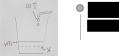
\includegraphics[width=0.8\textwidth]{figures/ODE.pdf}
    \caption{\label{fig:ode} Simple settings that are naturally described by an ordinary differential equation. Left: our simple bucket analogy. Right: a particle moving with velocity $v$.}
\end{figure}

Since differential equations describe how quantities are changing, we can calculate the quantity at a future time point by summing up the changes over time.
In a single time step $\Delta t$ the water level changes as
\begin{equation}
    \label{eq:ODE_step}
    y(t_0 + \Delta t) = y(t_0) + \Delta t \alpha
\end{equation}
where we used the symbol $\alpha$ to denote the influx rate that was 10 ml/s above.
Adding many contributions from such little steps, we can calculate the level at time $t$:
\begin{equation}
    y(t) = y(t_0) + \sum_{i=0}^n \Delta t \alpha
\end{equation}
where $\Delta t = (t-t_0)/n$, that is we split the interval $t-t_0$ into $n$ little steps.
Note that in the above equation, the rate $\alpha$ could change over time:
\begin{equation}
    y(t) = y(t_0) + \sum_{i=0}^n \Delta t \alpha(t_0 + i\Delta t)
\end{equation}
By making $n$ larger and $\Delta t$ smaller, we arrive at an integral over $t'$ from $t_0$ to $t$:
\begin{equation}
    y(t) = y(t_0) + \int_{t_0}^t \alpha(t')\, dt'
\end{equation}

So far, this example has been simple enough that we knew the solution to problem from the beginning and the formalism of ODEs might seem unnecessary.
But let's make this problem slightly more complex and assume the bucket is leaking and the amount of water that leaks is proportional to the pressure and thus to the water level $y(t)$ itself.
In other words, the bucket looses water at a rate $\beta y(t)$, where $\beta$ is the leakage rate.
This additional ``process'' (the leak) can be easily added to the differential equation:
\begin{equation}
    \label{eq:bucket}
    \frac{dy}{dt} = \alpha - \beta y(t)
\end{equation}
The solution to this equation is not quite as easy to guess, but the equation tells us a lot about the system.
The left panel of Fig.~\ref{fig:fixed_points} shows the right hand side of this equation (the rate of change of $y$) as a function of $y$.
For $y<\alpha/\beta$, the influx $\alpha$ is bigger than the leak $\beta y$ and the water level $y$ increases.
Otherwise, the leak is bigger than the efflux and $y$ decreases.
Thus from both sides, the system is driven against $y^* = \alpha/\beta$, which is a \textbf{stable fixed point} of the system.

\begin{figure}
    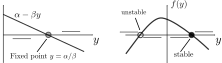
\includegraphics[width=0.8\textwidth]{figures/fixed_points.pdf}
    \caption{\label{fig:fixed_points}Left: Summary of the dynamics of the ODE in Eq.~\ref{eq:bucket}. Right: Stable and unstable fixed points of a generic time independent one dimensional dynamical system.}
\end{figure}

The qualitative analysis above has characterized the most important aspects of the system without actually solving the ODE.
There are many methods for solving ODEs explicitly, but often analysis like the one above or numerical solutions (discussed below) are more useful.
In this case, the system (`leaky bucket') has the solution
\begin{equation}
    y(t) = y_0 e^{-\beta t} + \frac{\alpha}{\beta}\left(1 - e^{-\beta t}\right)
\end{equation}
The initial condition $y_0$ and any deviation from the fixed point decay exponentially with rate $\beta$.
The correctness of this solution can be confirmed by differentiation.

\section{Numerical solutions of differential equations}
Eq.~\ref{eq:ODE_step} describes how the quantity $y$ changes in a small discrete time step $\Delta t$.
Numerical solutions of ODEs work essentially like this: adding small little increments to the solution until time has advanced sufficiently.
\begin{minted}{python}
    y, t = y0, t0            # define initial condition
    tmax, dt = 10, 0.1       # define final time and time step
    while t<tmax:            # loop until tmax and increment t and y
        t += dt
        y += dt*(alpha - beta*y)
\end{minted}
After this code has executed, $y$ will be the approximate solution of Eq.~\ref{eq:bucket}.
The smaller we choose $dt$, the more accurate the solution will be.
This method to solve the equation is often called the ``forward Euler'' method.
It is the simplest, and least accurate, method to solve differential equations.
For our purposes, it will often be good enough.
More complex methods are implemented in libraries which we will explore later in the course.
Please have a look at the accompanying notebooks for code and examples on these numerical solutions.

\section{Motion of particles and Newton's law}
Newton's law of motion
\begin{equation}
    F = m\times a
\end{equation}
is a differential equation. The acceleration $a$ is the rate at which the velocity changes.
The velocity $v$ is the rate at which the position $x$ of a particle changes.
Newton's law is thus not just one, but two coupled differential equations
\begin{equation}
    \begin{split}
        \frac{dx}{dt} & = v \\
        \frac{dv}{dt} & = a = \frac{F}{m} \\
    \end{split}
\end{equation}
The force $F$ can take different form in different problems.

A constant force, for example gravitational force, results in a steadily increasing velocity $v = \frac{Ft}{m}$ (exactly like the bucket without a leak).
This means the position is changing faster and faster with time
\begin{equation}
    \frac{dx}{dt} = \frac{Ft}{m}
\end{equation}
You can readily verify that the solution to this is $x(t) = x_0 + \frac{Ft^2}{2m}$.

Under the gravitational force of the earth, $F = m g$ where $g = 9.81 m/s^2$ and we obtain the familiar results $x(t) = x_0 = \frac{g ^2}{2}$. Note that the mass $m$ cancels.

\subsection{Harmonic oscillator}
Now consider a particle attached to a spring such that the force acting on the particle is $F = -\gamma x$.
This means that for $x>0$, the force is pulling to the left (towards smaller $x$) and in the opposite direction for $x<0$.
Such a situation is similar to a pendulum, a marble in a bowl, or a particle in a laser trap (optical tweezer) used for single molecule experiments (see Fig.~\ref{fig:harmonic}).
In addition to this force acting on the particle, there might also be a friction force.
Friction is typically proportional to the velocity itself $\eta v$.
Combining these two contributions, we find that this system is described by
\begin{equation}
    \label{eq:harmonic}
    \begin{split}
        \frac{dx}{dt} & = v \\
        \frac{dv}{dt} & = -\frac{1}{m} \left( x\gamma +  \eta v\right)\\
    \end{split}
\end{equation}
This system of equations can be solved exactly, but we will explore the solution numerically instead.
This numerical solution can be down for two variables $x$ and $v$ just like we did it for one variable above, see notebooks for details and Fig.~\ref{fig:harmonic} for the result.

The solution in Fig.~\ref{fig:harmonic} shows the trajectories for different levels of friction $\eta$.
This friction is one of the main aspects in which dynamics of large bodies differ from biological system at the micrometer scale.
For the motion of planets, friction can be neglected.
For everyday objects, friction is important, but often a perturbation rather than the dominating force. Nevertheless, objects tend to come to a resting states eventually due to friction.
The smaller the objects, the smaller their mass and friction becomes more important.
With increasing friction, the harmonic oscillator goes from eternal oscillations, to decaying oscillations, to a very slow relaxation.

\begin{figure}
    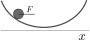
\includegraphics[width=0.4\textwidth]{figures/harmonic.pdf}
    \includegraphics[width=0.55\textwidth]{figures/harmonic_traj.pdf}
    \caption{\label{fig:harmonic}Left: Sketch of a particle moving along direction $x$ in a harmonic potential. Right: Trajectories of the particle at different levels of friction $\eta$.}
\end{figure}


\subsection{Over-damped dynamics}
On the micrometer scale, masses are tiny and friction is typically completely dominating the dynamics.
To explore the consequences of this observation, let's rewrite the second part of Eq.\ref{eq:harmonic} (with $F=-\gamma x$) by multiplying both sides by the mass $m$:
\begin{equation}
    m\frac{dv}{dt} = F - \eta v
\end{equation}
For very small $m$, the left hand side is close to $0$ and hence it follows that the velocity is $v \approx F/\eta$.
In other words, the velocity is the instantaneous ratio of force and friction.
In this over-damped limit, the equation of motion simplfies to
\begin{equation}
    \frac{dx}{dt} = \frac{F}{\eta} = -\frac{\gamma x}{\eta}
\end{equation}
whose solution is a simple exponential decay $x(t) = x_0 e^{-t \gamma/\eta}$.

\subsection{Friction and Stokes' law}
\label{sec:stokeslaw}
Friction in liquid medium is determined by the viscosity of the medium.
Viscosity is something we understand well from everyday life (water, oil, honey all have clearly different viscosity).
For the precise definition of viscosity, one usually considers the configuration in Fig.~\ref{fig:viscosity}.
The force required to move the plate is proportional to their area $A$ and the velocity gradient $v/d$ between the plates.
The constant of proportionality defines the viscosity
\begin{equation}
    F \sim \frac{Av}{d}  \quad \Rightarrow \quad F  = \eta \frac{Av}{d}
\end{equation}
Viscosity has dimension
\begin{equation}
    [\eta] = \left[ \frac{Fd}{Av}\right] = \frac{energy \times time}{volume} = \frac{force \times time}{area}
\end{equation}

Viscosity is typically measured in $N s/m^2$ and relevant values for us are
\begin{itemize}
    \item water: $0.001 \frac{Ns}{m^2}$
    \item cytosol: $0.003 \frac{Ns}{m^2}$
\end{itemize}



\begin{figure}
    \includegraphics[width=\textwidth]{figures/viscosity.png}
    \caption{\label{fig:viscosity}Viscosity is defined via the force required to move two plates with area $A$ at distance $d$ relative to each other with velocity $v$.}
\end{figure}

\section{Growth processes in biology}

\subsection{Exponential Growth}
see notebooks

\subsection{Logistic Growth}
see notebooks

\subsection{Ecological dynamics}
see notebooks

\subsection{Infectious disease dynamics}
see notebooks




 %!TEX root = main.tex
\chapter{Models of gene regulation}

The expression of genes is tightly regulated in space and time.
One important mechanisms of gene regulation is through proteins called transcription factors that bind to specific sequences in the genome and activate or repress transcription of a nearby gene.
By combining multiple transcription factors, complicated combinatorial logic can be implemented.
Accurate regulation requires that transcription factors find their target sites reliably despite being at low concentration and the fact that the genome is wrapped around histones and coiled up in higher order chromatin structures (at least in eukaryotes).
Fig.~\ref{fig:TF_abundance} shows that in E.~coli activators (factors that increase expression) are typically present between 1 and 100 times while repressors about 10 times more abundant.
In this chapter, we will discuss simple models involving gene regulation and will draw on our previous discussions of diffusion and polymers.


\begin{figure}[tb]
	\centering
	\includegraphics[width=0.9\textwidth]{figures/TFCopyNumber_bionumbers.png}
	\caption{Abundance of transcription factors in E.coli. From \href{http://book.bionumbers.org/what-are-the-copy-numbers-of-transcription-factors/}{bionumbers.org} with original data from \citep{li_quantifying_2014}. The data are shown as a cumulative distribution, that is the y-axis show the fraction of transcription factors that have an abundance below the value on the x-axis. Cumulative distributions might be a little unfamiliar to read, but have many advantages over classical histograms since they don't require a choice of binning.}
	\label{fig:TF_abundance}
\end{figure}

\section{DNA-transcription factor binding}
Given a TF is at a certain concentration and has a specific target sequence, what fraction of the time is the target sequence occupied?
This is analogous to the population of the transition state in Michaelis-Menten kinetics (page 115 in Hiller's script):
\begin{equation}
P(TF\,bound) = \frac{[X]}{K + [X]}
\end{equation}
where $[X]$ is the concentration of the TF.
The analog of the concentration of the enzyme is the DNA binding site concentration which is fixed and absorbed into $K$.
With increasing concentration, the occupation probability goes up and saturates at 1.
More often than not, transcriptional regulation is cooperative and involves multiple TFs (the same or different types).
This situation is analogous to cooperative binding of oxygen to hemoglobin: each TF individually binds to the DNA and they enhance the probability to remain bound by binding to each other.
Consider two transcription factors A and B with TF-DNA interaction free energies $\epsilon_A$ and $\epsilon_B$ and a TF-TF interaction of $J_{AB}$.
The grand partition function is then (comp.~page 78 of Hiller's script)
\begin{equation}
	\mathcal{Z} = 1 + ([A]/k_A) e^{-\epsilon_A/kT} + ([B]/k_B) e^{-\epsilon_B/kT} + ([A][B]/k_Ak_B)e^{-(\epsilon_A+\epsilon_B+J_{AB})/kT}
\end{equation}
Pulling out the concentrations, the probability that both A and B are bound is
\begin{equation}
	P_{AB} = \frac{[A][B]e^{-(\epsilon_A+\epsilon_B + J_{AB})}}{k_Ak_B +\cdots+ [A][B]e^{-(\epsilon_A+\epsilon_B+ J_{AB})}}
\end{equation}
For strongly cooperative systems, the states where only a fraction of the factors are bound don't contribute much and are often ignored.
Approximately, one has the following
\begin{equation}
	P_{AB} \approx \frac{[A][B]e^{-(\epsilon_A+\epsilon_B + J_{AB})}}{k_Ak_B + [A][B]e^{-(\epsilon_A+\epsilon_B+ J_{AB})}} = \frac{[A][B]}{K + [A][B]}
\end{equation}
where we absorbed the exponential factor into $K$.
This form of cooperative binding generalizes to $m$ copies of A and $m$ copies of $B$ as follows.
\begin{equation}
	P_{AB} \approx \frac{[A]^m[B]^n}{K + [A]^m[B]^n}
	\label{eq:hill}
\end{equation}
Here, it is important to realize that the units of $K$ change as $m$ and $n$ change, but the structure of the denominator is always the same:
$K$ is proportional to the probability of the unbound state, $[A]^m[B]^n$ is proportional to the bound state.
Curves like the ones in Eq.\ref{eq:hill} are known as Hill curves and $m$ and $n$ are Hill-coefficients (normally Hill curves consider only one species $A$ and only one coefficient $m$).
The higher the Hill-coefficient, the more cooperative and steep in the binding curve, see Fig.~\ref{fig:hill}.
Highly cooperative regulation can there yield to an almost switch like-response.

\begin{figure}[tb]
	\centering
	\includegraphics[width=0.48\textwidth]{Hill_curve.png}
	\includegraphics[width=0.48\textwidth]{null_clines.pdf}
	\caption{Left: Hill curves at different levels of cooperativity.
			Right: Null clines of the simple auto-activator system in Eqs.\ref{eq:act_mRNA} and \ref{eq:act_protein}. Units of time and concentrations are chosen such that $\alpha=\beta=1=K=1$, $n=4$, $\gamma=2, \delta=1$.}
	\label{fig:hill}
	\label{fig:null_clines}
\end{figure}


\section{Simple genetic circuits}
Which genes are transcribed at which rate at a given time is a function of the concentration of regulatory proteins, RNA polymerase, epigenetic modifications etc. -- essentially a function of the state of the cell.
To study gene expression using computational models, we will typically try to isolate the most important factors into a simple model and describe their dynamics by a system of differential equations:
\begin{eqnarray}
	\frac{d x_1}{dt} &=& f_1(x_1, x_2, \ldots, x_n, t) \\
	\frac{d x_2}{dt} &=& f_2(x_1, x_2, \ldots, x_n, t) \\
	\vdots & = & \vdots \\
	\frac{d x_n}{dt} &=& f_n(x_1, x_2, \ldots, x_n, t)
\end{eqnarray}
Here the functions $f_i(x_1,\ldots, x_n,t)$ describe how rapidly quantity $i$ is produced given the state of the cell.
This function could depend explicitly on time, for example because of daily rhythms.
Such computational models of gene expressions fall into the domain of dynamical systems.
A very good and accessible introduction to dynamical systems is the book by Steven Strogatz \citep{strogatz_nonlinear_2014}.

The simplest dynamical systems are one-dimensional and of the form
\begin{equation}
	\frac{dx}{dt} = f(x)
\end{equation}
In the case of gene expression modeling, the function $f(x)$ typically consists of a production term and a degradation term, for example like the following:
\begin{equation}
	\frac{dx}{dt} = \alpha - \beta x
\end{equation}
In this case, $x$ is produced at constant rate $\alpha$ and decays with rate $\beta$.
The concentration $x$ is going to increase whenever $\alpha > \beta x$ and decrease when $\alpha <\beta x$.
The system has hence a fixed point $\bar{x} = \alpha/\beta$.

\subsection*{Self activation:}
The simplest genetic circuits are genes that regulate their own expression.
We will first consider a gene $x$ whose transcription is regulated by its own product protein $X$.
To keep the notation simple, lets denote the mRNA concentration by $x$ and that of the protein by $X$.
mRNA is produced whenever the promoter is occupied by $n$ copies of protein $X$ and decays in a linear fashion.
\begin{equation}
\label{eq:act_mRNA}
	\frac{dx_1}{dt} = \alpha\frac{x_2^n}{K+x_2^n} - \beta x_1
\end{equation}
The parameters $\alpha$ and $\beta$ are the transcription rate and mRNA decay rates, respectively.
The mRNA is then translated to proteins such that the protein concentration evolves as
\begin{equation}
\label{eq:act_protein}
	\frac{dx_2}{dt} = \gamma x_1 - \delta x_2
\end{equation}
Here, $\gamma$ is the translation rate (the amount of protein produced by mRNA per unit of time) and $\delta$ is the degradation rate.

To a qualitative idea of the behavior of the behavior of the system, it is useful to graph the lines at which $\frac{dx_1}{dt}=\frac{dx_1}{dt}=0$.
For Eqs.\ref{eq:act_mRNA} and \ref{eq:act_protein} this results in $x_1=\delta/\gamma x_2$ and $x_1 = \frac{\alpha}{\beta}\frac{x_2^n}{K+x_2^n}$.
These lines are known as null clines are shown in Fig.~\ref{fig:null_clines}B.
Whenever the null-clines intersect, the system is at a fixed point, that is a point where the concentrations don't change.
Some of these fixed points are stable and other unstable.
A stable fixed point ``attracts'' solutions in its neighborhood, and trajectories in the vicinity of an unstable fixed point move away from the fixed point.

In the case shown in Fig.~\ref{fig:null_clines}B, there are two stable fixed points separated by one unstable fixed point.
Such systems are called bistable.
Each of the stable fixed point has a ``basin of attraction''.
Any simulation with initial condition in the basin of attraction of one fixed point will flow towards that fixed point.
Simulations of this case are shown in Fig.~\ref{fig:bistable}.

\begin{figure}[tb]
	\centering
	\includegraphics[width=\textwidth]{two_stable_fixed_point}
	\caption{An auto-activator with sufficiently strong cooperativity is bistable. Depending on the initial condition, the system flows towards an ``on'' or ``off'' state}
	\label{fig:bistable}
\end{figure}


\subsection*{Self repression}
Above, we considered the case of a gene product activating its own transcription and activation was modeled as Hill-function.
Repression works analogously, but the gene is transcribed with the repressor site is unbound and silent whenever a repressor is bound.
So instead of being proportional to $X^n/(K+x_2^n)$, transcription is now proportional to
\begin{equation}
	1-\frac{x_2^n}{K+x_2^n}=\frac{K}{K+x_2^n}
\end{equation}
The differential equations describing the dynamics are therefore
\begin{eqnarray}
	\label{eq:repressor}
	\frac{dx_1}{dt} &= \alpha\frac{K}{K+x_2^n} - \beta x_1 \\
	\frac{dx_2}{dt} &= \gamma x_1 - \delta x_2
\end{eqnarray}
This system has only one stable fixed point when repression and production are in balance.
Fig.~\ref{fig:repressor} show the dynamics of such a system.
Such auto-repressor systems are well suited to maintain the concentration of a species at a particular value: They work essentially like thermostats on a radiator.

Systems with negative feedback have a tendency to oscillate.
The example in Fig.~\ref{fig:repressor}, however, doesn't yet show autonomous oscillations.
To construct a true oscillator, one either needs an additional component or a stronger non-linearly/cooperativity.

\begin{figure}[tb]
	\centering
	\includegraphics[width=\textwidth]{spiral_fixed_point.pdf}
	\caption{Dynamics of an auto-repressor. In this example, $\gamma=2.2$, $\delta=1$, and $n=4$.}
	\label{fig:repressor}
\end{figure}

\subsection*{Stochasticity in gene expression}
Fig.~\ref{fig:TF_abundance} shows that many TFs are present in small numbers in the cell.
As a result, the degradation or production of one TF molecule can make a substantial difference to the dynamics.
Since all molecular process are stochastic, we expect that expression of many genes and the levels of the corresponding proteins to fluctuate.

To model stochastic gene expression dynamics, one re-interprets the concentration variables as molecule numbers and the different terms in the ODEs as rates of Poisson processes.
After replacing $x$ by a discrete particle number $n$ and appropriate rescaling of the rate constants (we changed units from concentrations to particle numbers), the different terms can be interpreted as \emph{probability of a reaction per unit time}.
Given the degradation term $\delta n$, for example, the probability that $m$ particles were degraded in time interval $\Delta t$ is Poisson distributed with mean $\Delta t \delta n$.
The particle numbers can then be updated in small time steps similar to the forward Euler scheme used for deterministic ODEs in the lecture.
Note, however, that stochastic models of gene expressions are an active field of research with many sophisticated techniques to make such simulations accurate and fast.



% random walks and diffusion
 %!TEX root = main.tex
\chapter{Random walks and diffusion}

In absence of active transport, microscopic objects move due to ubiquitous thermal motion:
Every molecule jitters around in random ways and the sum of the many kicks and pushes causes an erratic movement known as \href{https://en.wikipedia.org/wiki/Brownian_motion}{Brownian motion}.
It is named after Robert Brown who noticed that pollen grains jitter when observing them in a microscope.
Such Brownian motion or diffusion is the primary mode at which nutrients, signaling molecules, and proteins move around in bacterial cells.
In this chapter, we will explore the basic properties of diffusion and how it depends on the size of the particles, the viscosity of the medium, and temperature.

Getting a sense of the time scales over which molecules diffuse certain distances is crucial for a quantitative understanding of many biological process.
The process of diffusion of molecules in the cytosol can be studied and quantified using the technique \href{https://en.wikipedia.org/wiki/Fluorescence_recovery_after_photobleaching}{``Fluorescence Recovery After Photobleaching''} (FRAP), see Fig.~\ref{fig:FRAP}
Say you labeled your molecule of interest with a fluorescent protein (GFP) that bleaches due to photo damage in strong illumination.
If you now bleach the dye in some fraction of your field of view, you have set up a sharp gradient between fluorescent and non-fluorescent versions of your molecule.
The recovery of the fluorescence signal is due to diffusion of intact GFP molecules into the space that was bleached.
This fluorescent recovery is very smooth and deterministic, despite the fact that the motion of the individual particles is completely erratic and random.
This is just one example how the net effect of many random events gives rise to behavior that is simple and smooth.
We will explore how this comes about in the next section.

\begin{figure}[tb]
	\centering
	\includegraphics[width=\textwidth]{FRAP.png}
	\caption{The top left image shows a cell with GFP at homogeneous concentration in the cytosol. After bleaching (destroying) the fluorescent proteins in small volume with a high intensity laser, fluorescence recovers overtime through diffusion of intact GFP into the bleached volume.  Image source: bioquant Heidelberg}
	\label{fig:FRAP}
\end{figure}

\section{Random walks in one dimension}
Consider an object on a track that moves by a fixed distance every second.
With probability $p$ is moves to the right and with probability $q=1-p$ it moves to the left.
How far do expect this object to be after $n=1,10,100,\dots$ steps?
This simple example has a closed solution, but we will explore this with a little simulation before going into the math.
Take a look at the little code snippet \ref{lst:random_walk}.
This code generates a couple of random walks and graphs them.
A typical output is shown in Fig.~\ref{fig:RW}.

\begin{listing}[h]
\inputminted{python}{scripts/random_walk.py}
\caption{Script that generates and plots random walks.}
\label{lst:random_walk}
\end{listing}

\begin{figure}[tb]
	\centering
	\includegraphics[width=0.48\textwidth]{figures/random_walk.pdf}
	\includegraphics[width=0.48\textwidth]{figures/random_walk_histogram.pdf}
	\caption{Left: 5 realizations of a random walk with $p=0.53$. Right: Histograms of the position of random walks after $n=10, 30, 100$ steps. The histograms are getting wider and slowly move to the right. }
	\label{fig:RW}
\end{figure}

After having explored such random walks in simulations, let's look at them more systematically.
The probability of a particular sequence of left/right steps is $p^k q^{n-k}$, where $k$ is the number of steps to the right and $n-k$ is the number of steps to the left.
Now there is exactly one way of taking $n$ out of $n$ steps to the right or left, but there are many ways of doing some mix of right/left steps.
In fact, the number of ways to walk $k$ steps to the right and $n-k$ steps to the left is given by
\begin{equation}
	C_n^k = \frac{n!}{k!(n-k)!} = { n\choose k}
\end{equation}
This is known as the binomial coefficient and should be familiar from high-school.
The factorial $n! = n(n-1)(n-2)\cdots 2\cdot1$
The probability of observing the random walk at position $k$ is therefore given by
\begin{equation}
	P_n^k = p^kq^{n-k}\frac{n!}{k!(n-k)!}
\end{equation}
which is known as the Binomial Distribution.

\subsection{Mean and variance of a random walk}
On average, the random walker will move to the right if $p>q$, to the left if $p<q$, and no net movement is expected if $p=q=0.5$.
This intuition is confirmed by a short calculation.
The number of steps to the right is given by
\begin{equation}
\begin{split}
	\langle k \rangle & = \sum_{k=0}^n k P_n^k = \sum_{k=1}^n \frac{n!}{(k-1)! (n-k)!} p^k q^{n-k} \\
	&= np \sum_{k=1}^n \frac{(n-1)!}{(k-1)! (n-k)!} p^{k-1} q^{n-k} = np
\end{split}
\end{equation}
where the last equality used the fact that summand is again a binomial distribution $P(k-1, n-1)$ and hence the sum evaluates to one.
After $n$ steps, the walker has therefore taken on average $np$ steps to the right and $nq$ steps to the left and the average position is therefore $n(p-q)$.

This calculation established that the mean position of the random walker is $\langle x\rangle = n(p-q)$, but random walkers are not moving deterministically along the mean.
Instead, some will be on the left, some of the right of $\langle x\rangle$.
To quantify the spread of a random walk, we calculate its variance.
The variance is defined as the mean squared distance from the mean and we will first calculate the variance in the number of steps to the right.
The details of this calculation are a little tedious, but straightforward, and I provide them at the end of this chapter:
\begin{equation}
	\langle (k - np)^2 \rangle = \sum_{k=0}^n k^2 P_n^k - n^2p^2 = npq
\end{equation}
Since the $x=2k-n$ we immediately find $var(x) = 4npq$.
Note that this is the average squared deviation from the mean.
The typical distance from the mean is therefore the square root $\delta x \sim 2\sqrt{npq}$.
The fact that the typically spread of the random walker increases with the square root of the number of steps has far reaching implications.
In particular, the random component of the motion dominates initially
\begin{equation}
	2\sqrt{npq} > n(p-q) \quad \Rightarrow \quad n < \frac{4pq}{(p-q)^2}
\end{equation}
The smaller the difference between $p$ and $q$, the longer the random part dominates.
If $p$ is very close to $q$, the random part dominates for a very long time!
The fact that random components depend on the square root of the number events/steps/experiments while the deterministic part is linear in this number is the basis of almost all statistical tests and you will encounter this relationship over and over again.

It is important to realize that in most situations, the probability to move to the right or the left are exactly the same: When there is no force pulling the molecule in a particular direction, thermal noise will move it in every direction with equal rate.
In this case, $\langle x \rangle = 0$ no matter how long you wait and the only contribution to a molecules motion is the random component $2\sqrt{npq}$.

\subsection{From random walks to diffusion}
So far, we discussed the properties of random walks on a discrete one dimensional grid.
The equation describing the distribution of this random walk can be rewritten as
\begin{equation}
	P(x,n) = p P(x-1,n-1) + q P(x+1,n-1)
\end{equation}
This equation describes how the probability of finding the walker at position $x$ changes with every step: the first term involves a step to the right which happens with probability $p$, the second term corresponds to a step to the left.

\begin{figure}[tb]
	\centering
	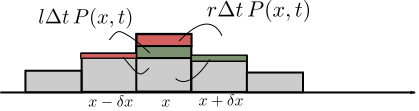
\includegraphics[width=0.6\columnwidth]{figures/RW_masterEq}
	\caption{Schematic of the dynamics of the distribution $P(x,t)$ of the
	position of a diffusing substance. The center bin at $x$ looses mass to the left (red) and right (green) but gains from the bins at $x\pm \delta x$. The neighboring bins, however, are smaller and $P(x,t)$ will therefore decrease. The diffusion equation is obtained by reducing $\delta x$ and $\Delta t$ gradually to 0.}
	\label{fig:masterEQ}
\end{figure}

In a biological system, there are no discrete time points and a molecule will move due to thermal motion by a random distance.
But we can approximate this situation by making the time and spatial steps smaller and smaller.
We will from now on replace $n$ by time $t$ and treat the position $x$ as a continuous variable.
In a time interval $\Delta t$, the molecule receives kicks that push it to the right of left by a distance $\delta x$ with probability $r\Delta t$ and $l\Delta t$.
\begin{equation}
	P(x,t+\Delta t) = (1-(r+l)\Delta t) P(x,t) + r\Delta t P(x-\delta x, t) + l\Delta t P(x+\delta x,t)
\end{equation}
The first term on the right hand side corresponds to cases where the molecular stays where it is.
The second and third term correspond to jitter to the right and left, respectively (see Figure \ref{fig:masterEQ}).
This equation can be rearranged slightly
\begin{equation}
	\frac{P(x,t+\Delta t) - P(x,t)}{\Delta t} = -(r+l) P(x,t) + r P(x-\delta x, t) + l P(x+\delta x,t)
\end{equation}
which should remind you of a differential equation.
Rearranging this a little more, we find
\begin{equation}
\begin{split}
	\label{eq:discrete_update}
	\frac{P(x,t+\Delta t) - P(x,t)}{\Delta t} = &\frac{\delta x^2(r+l)}{2} \frac{P(x+\delta x,t) - 2 P(x,t) +P(x-\delta x, t)}{\delta x^2}\\&
	 - \delta x (r-l) \frac{P(x+\delta x, t) - P(x-\delta x,t)}{2\delta x}
\end{split}
\end{equation}
The terms on the right hand site are discrete second and frist derivatives (see \href{https://en.wikipedia.org/wiki/Finite_difference}{Finite differences} on wikipedia).
Defining the diffusion coefficient $D=\frac{\delta x^2 (r+l)}{2}$, the drift velocity $v=\delta x (r-l)$, and taking the limit of small space and time steps, we arrive at
\begin{equation}
\label{eq:diffusion}
	\frac{\partial P(x,t)}{\partial t} = D\frac{\partial^2 P(x,t)}{\partial x^2} - v \frac{\partial P(x,t)}{\partial x}
\end{equation}
This equation is called diffusion equation and describes transport in many biological systems -- it is also known as the heat equation as it describes the flow of heat in a solid.
This type of equation is called a partial differential equation -- something you might not have come across in previous courses.
The concept is not very difficult, but the different notations that are used for such equations can be confusing (see \href{https://en.wikipedia.org/wiki/Partial_derivative}{wikipedia on partial derivatives}).

The object $P(x,t)$ can be interpreted as the density of molecules at position $x$ and time $t$.
This density changes due to diffusion of the molecules according to Eq.~\ref{eq:diffusion}.
For the following discussion, we will assume that $v=0$, that is there is no directed motion.
In this case, density increase were curvatures is positive and decreases where it is negative.
In other words, ``hills'' decrease and ``valleys'' are filled.

The diffusion constant $D$ has units of length${}^2$/time, e.g.~m$^2$/s.
Even though the diffusion constant determines how rapidly molecules spread, it is not a velocity which would have units m/s.
The crucial difference is that diffusion describes \emph{undirected} motion, while velocities describe directed motion.
Undirected motion has to be characterized in terms of the squared displacement since the net displacement vanishes.


\subsubsection{Solutions to the diffusion equation}
In our discussion of discrete random walks, we showed that the binomial distribution describes the position of the walker after $n$ steps.
You might know that the continuous analog of the binomial distribution is the {\it Gaussian} or {\it Normal} distribution.
A normal distribution (centered around $x=0$) with variance $\sigma^2$ is given by
\begin{equation}
	N(x | \sigma) = \frac{1}{\sqrt{2\pi \sigma^2}} e^{\frac{x^2}{2\sigma^2}}
\end{equation}
The normal distribution is a solution to the diffusion equation with
\begin{equation}
	\sigma^2 = 2Dt
\end{equation}
This can be readily verified by direct computation and is done explicitly at the end of this chapter.

\subsubsection{Numerical solution of the diffusion equation}
In many cases, analytical solution of the diffusion equation is not possible and one instead resorts to numerical methods.
Numerical solutions essentially work with the discrete approximation Eq.~\ref{eq:discrete_update}.
The hopping rates $r$ and $l$ depend on $D$ and $v$ (independent of the discretization) and the spatial discretization:
\begin{equation}
	D = \frac{r+l}{2}\delta x^2 \quad \mathrm{and} \quad v =(r-l)\delta x
\end{equation}
is readily solved for $r$ and $l$
\begin{equation}
	l = \frac{D}{\delta x^2}- \frac{v}{2\delta x}\quad \mathrm{and} \quad
	r = \frac{D}{\delta x^2} + \frac{v}{2\delta x}
\end{equation}

\subsection{Typical diffusion coefficients in cells}

\begin{itemize}
  \item GFP in eukaryotic cells: $\sim 25 \mu m^2/s$
  \item GFP in prokaryotic cells: $\sim 10 \mu m^2/s$
  \item mRNA (actin in mouse): $\sim 0.2 \mu m^2/s$
  \item $\mathrm{H_2O}$ molecule in $\mathrm{H_2O}$: $\sim 2000 \mu m^2/s$
  \item $\mathrm{H^+}$ molecule in $\mathrm{H_2O}$: $\sim 7000 \mu m^2/s$
\end{itemize}


\subsubsection{How long does it take for a protein to diffuse a distance $x$?}
The typical distance scale after a time $t$ is
\begin{equation}
	\Delta x = \sqrt{2Dt} \quad \Rightarrow \quad t = \frac{\Delta x^2}{2D}
\end{equation}

\begin{itemize}
  \item $\Delta x = 1\mu m$: $t = 0.05s$ [across a bacterium]
  \item $\Delta x = 10\mu m$: $t = 5s$   [across a eukaryotic cell]
  \item $\Delta x = 1000\mu m$: $t = 5000s=83m$
  \item $\Delta x = 1m$: $t = 5\times 10^9s=160y$   [along a peripheral axon]
\end{itemize}
Hence diffusion is fast on short distances, but completely inadequate on long distances.


\section{Fluxes}
Much transport in biology is diffusive: Many enzymatic rates are diffusion limited and processes like nuclear import involves diffusion through the nuclear pore (facilitated by suitable transport proteins).
We will now explore different ways in which diffusion is mediating and limited such rates.

Consider the set-up illustrated in Fig.~\ref{fig:diffusive_transport} of a long narrow channel with a high concentration on the left and a low concentration on the right.
If the channel is narrow and the reservoirs on the left and right large, we expect an approximately homogeneous concentration in both reservoirs and a steady concentration gradient across the channel.
The diffusion of molecules in our system is governed by the diffusion equation and we there expect that the should be a solution to the diffusion equation that (i) does not depend on time ($P(x,t)=P(x)$), and (ii) that is high on the left, low on the right, and has a gradient in the middle.
The only spatial direction that is relevant in Fig.~\ref{fig:diffusive_transport} is the $x$ axis and we will ignore slight variation long the $y$ and $z$ axes.
A time invariant solution implies
\begin{equation}
	\frac{\partial P(x,t)}{\partial t} = 0 = D\frac{\partial^2 P(x,t)}{\partial x^2} = 0
\end{equation}
This equation tells us two things: (i) the solution has to be independent of $t$, and (ii) is has zero curvature in $x$.
Zero curvature implies that the solutions are linear.
Inside the channel, we therefore have
\begin{equation}
 	P(x) = P^l + \frac{(P^r-P^l)x}{L} \ ,
\end{equation}
where $P^l$ and $P^{r}$ are the concentrations on the left and right while $L$ is the length of the channel and $x$ is the coordinate along the channel $x\in [0,L]$.
Our intuition already tells us that in a set-up like Fig.~\ref{fig:diffusive_transport} material will flow from left to right, that is the concentration on left will decrease slowly while that on the right will increase (in analogy to temperature equilibration).
To calculate this flux, it is useful to rewrite the diffusion equation
\begin{equation}
	\frac{\partial P(x,t)}{\partial t} = -\frac{\partial }{\partial x}\left[-D\frac{\partial P(x,t)}{\partial x} \right] = - \frac{\partial }{\partial x} j(x,t)
\end{equation}
The object in brackets is known as the flux $j(x,t)$.
Once broken down like this, the diffusion equation is rather intuitive: the concentration changes in time if the flux changes in space.

In our case, the material transported across the channel is
\begin{equation}
	J = D\frac{P^l - P^r}{L}\times A
\end{equation}
where $A$ is the cross-sectional area of the channel.
Let's do a quick consistency check: $D$ has units $m^2/s$, concentrations have units $\mathrm{stuff}/m^3$, $L$ has units $m$ and $A$ has units $m^2$. Hence $J$ has units $\mathrm{stuff}/s$ which is exactly what we expect for a flux.

\begin{figure}[tb]
	\centering
	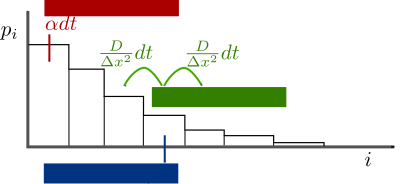
\includegraphics[width=\textwidth]{figures/diffusive_gradient.pdf}
	\caption{Diffusion through a narrow channel between two reservoirs results in a linear concentration profile along the channel.}
	\label{fig:diffusive_transport}
\end{figure}

\subsubsection*{Transport through the nuclear pore}
With these results, we can now estimate the number of molecules that transverse the nuclear pore per second given a concentration gradient.
The center of the nuclear pore has a diameter of about 30nm and a height of about 30nm.
A typical protein has a diffusion coefficient of about $10\mu m^2/s$.
Our expectation for the number of particle translocations is therefore
\begin{equation}
	J \approx \Delta C \times 0.025\mu m^3/s \approx 2.5\times 10^{-16}l/s \Delta C
\end{equation}
At a $\mu M$ concentration difference, this corresponds to a few hundred molecules per second.
There are extremely rough estimates and the medium inside the pore will have significant effects on this number, but we get a first idea.
For more detail on this problem, see this paper by \citet{ribbeck_kinetic_2001}.

\subsubsection*{Diffusion limited rates}
Many biochemical reactions are limited by the time it takes for the reactants to find each other.
Since the reactants move around by diffusion, such rates are called \emph{diffusion limited}.
In this case the activity of an enzyme, for example, cannot be increased by modifying the enzyme since the fundamental speed-limit is the arrival of the substrate.
The rate of reaction, however, will increase with the substrate concentration.
The full solution of this problem involves solving the diffusion equation in three dimensions.
While possible, we don't want to go into these technicalities here and simply state and motivate the result.
The diffusion limited rate between substance $a$ and substance $b$ is given by
\begin{equation}
	\label{eq:diffusion_limit}
	\kappa = 4\pi (D_a+D_b)(r_a+r_b) \ ,
\end{equation}
where $D_a$ and $D_b$ are the diffusion coefficients and $r_a$ and $r_b$ are the radii of the two reactants.
The sum of the two diffusion coefficients happens to be the diffusion of the relative distance between two molecules, and the sum of the radii is the minimal distance the two reactants have to attain to react.
The quantity $\kappa$ as units $m^3/s$, which becomes `particles per second' when multiplied by a concentration.

The situation above is quite idealized and additional factors, for example relative orientation, affect the actual rate.


\section{Diffusion coefficients and Stokes-Einstein relation}
There is simple law that relates the diffusion constant to other properties of the medium and the diffusion particles: this law is called the Stokes-Einstein relation.
Before we derive it, lets take a moment to think about which quantities might matter:
\begin{itemize}
  \item big things diffuse more slowly, hence the radius $r$ with units $length$ is important
  \item diffusion is thermal motion, hence $kT$ with units $energy$ should be relevant
  \item diffusion is slower at high viscosity, hence $\eta$ with units $Force\cdot time/area$ will matter.
  	(viscosity is the factor relating the force per unity area to the velocity gradient in fluid flow.)
\end{itemize}

How can we combine these quantities to give us a diffusion constant with units $length^2/time$?
Clearly, $\eta$ has to be in the denominator and $kT$ in the numerator. Their ratio has the following units:
\begin{equation}
\frac{kT}{\eta}\quad \mathrm{has\ units}\quad \frac{Force\cdot length\cdot area}{Force \cdot time} = \frac{length^3}{time}
\end{equation}
Hence $kT/\eta r$ has the right units and we expect the diffusion coefficient to scale as
\begin{equation}
D \sim \frac{kT}{\eta r}
\end{equation}
Let's see how this holds up when analyzing the problem more carefully.
Einstein considered diffusion in a general potential. We will assume here we have a harmonic potential $U(x) = \alpha x^2/2$, i.e., a force $F = \alpha x$ is pulling the particle back to $x=0$.
The motion of the particle is governed by the diffusion equation
\begin{equation}
\frac{\partial P(x,t)}{\partial t} = D \frac{\partial^2 P(x,t)}{\partial x^2} + \alpha \mu \frac{\partial P(x,t)}{\partial x}
\end{equation}
where $\mu$ is the mobility of the particle, i.e., the relationship between velocity and pulling force in viscous media. Mobility is the inverse of friction.
At steady state, the distribution of the particle is
\begin{equation}
P(x) = \frac{1}{\sqrt{2\pi D/\alpha}}e^{ - \frac{\alpha x^2}{2D}}
\end{equation}
However, the Maxwell-Boltzmann distribution requires that the equilibrium distribution is also proportional to $e^{-\alpha x^2/2kT}$. Hence we find
\begin{equation}
D = \mu kT
\end{equation}
This is one example of a fluctuation-dissipation relation that connects macroscopic quantities such as mobility with the microscopic quantities such as the diffusion coefficients.

Next, we need to consider how the mobility is related to the geometry of the particle and the solution.
This is given by Stokes' law (see Section \ref{sec:stokeslaw}) that relates the friction force to the size of the sphere and the viscosity:
\begin{equation}
\mu = \frac{1}{6\pi \eta r}
\end{equation}
Deriving this is a standard exercise in fluid dynamics, but nothing that we will go into here. Have a look at \href{https://en.wikipedia.org/wiki/Stokes%27_law}{the wikipedia page for Stokes' law} if you are curious.

Putting the Einstein relation and Stokes' law together, we obtain the Stokes-Einstein relation
\begin{equation}
D = \frac{kT}{6\pi \eta r}
\end{equation}
The remarkable fact about this equation is that $\eta$ can be measured at macroscopic scales and the microscopic structure does not feature explicitly. Nevertheless, together with the molecular radius and the energy scale $kT$, it determines the diffusion coefficient of microscopic particles.
Our intuitive scaling ansatz above was off by the factor $6\pi$, but did capture the essence of the problem.

The viscosity of water at room temperature is
\begin{equation}
\eta_0 = 0.001\frac{N s}{m^2} = 10^{-15}\frac{N s}{\mu m^2} = 10^{-3}\frac{pN s}{\mu m^2}
\end{equation}
The cytosol typically has a 3fold higher viscosity. So let's see how well the numbers given above compare to the prediction (Stokes' law assumes a perfect sphere, so we don't expect perfect agreement).
\begin{equation}
D = \frac{kT}{6\pi \eta} \frac{1}{r} \approx \frac{4pN \cdot nm \cdot \mu m^2}{20\cdot 3\cdot 10^{-3} pN s}\frac{1}{r} = \frac{1}{r} \frac{\mu m^3}{15s}
\end{equation}
For GFP with an radius of about 2nm, we find $D\approx 33 \mu m^2/s$ -- a little high but not too bad. For a water molecule with $r\approx 0.1 nm$, our predictions is $D = 660\mu m^2/s$ in the cytosol and $2000\mu m^2/s$ in pure water as expected.



\section{Derivations}

\subsection*{Variance of the binomial distribution}
\begin{equation}
	\begin{split}
	\langle (k - np)^2 \rangle & = \sum_{k=0}^n (k^2 - 2knp + n^2 p^2) P_n^k = \sum_k k^2 P_n^k - n^2p^2 \\ &
	= \sum_k (k(k-1) + k) P_n^k - n^2p^2 = np -n^2 p^2 + \sum_k k(k-1)\frac{n!}{k!(n-k)!}p^k q^{n-k} \\
	&= np - n^2 p^2 + n(n-1) p^2 \sum_{k=2}^n \frac{(n-2)}{(k-2)!(n-k)!} = np-np^2 = np(1-p) = npq
	\end{split}
\end{equation}
Note that the variance peaks at $p=0.5$ and goes to zero as $p$ approaches 0 or 1.


\subsection*{Gaussian solution to the diffusion equation}
Above, we asserted that
\begin{equation}
	P(x,t) = \frac{1}{\sqrt{4\pi Dt}}e^{-\frac{x^2}{4Dt}}
\end{equation}
solves the diffusion equation
\begin{equation}
	\frac{\partial P(x,t)}{\partial t} = D \frac{\partial^2 P(x,t)}{\partial x^2}
\end{equation}
Let's look at both sides of the equation separately.
\begin{equation}
\begin{split}
	D \frac{\partial^2 P(x,t)}{\partial x^2} & = -\frac{D}{\sqrt{4\pi Dt}}\frac{\partial}{\partial x}\frac{x}{2Dt} e^{-\frac{x^2}{4Dt}} \\
	&= -\frac{D}{\sqrt{4\pi Dt}}\left(\frac{1}{2Dt} - \frac{x^2}{4D^2t^2}\right) e^{-\frac{x^2}{4Dt}} =
	\left(\frac{x^2}{2D t^2} - \frac{1}{t}\right)\frac{e^{-\frac{x^2}{4Dt}}}{4\sqrt{\pi Dt}}\\
	\frac{\partial P(x,t)}{\partial t} &= \frac{e^{-\frac{x^2}{4Dt}}}{\sqrt{4\pi Dt}}\left(\frac{x^2}{4Dt^2}-\frac{1}{2t}\right)
\end{split}
\end{equation}
Left and right side of the equation are equal and the Gaussian with a variance that increases linearly in time solves the diffusion equation.



\chapter{Gene regulation in space and time}
% \section{Transcription factor search}
% In chapter 2, we discussed the rate at which two molecules encounter each other by diffusion and derived the diffusion limit to association (see Eq.~\ref{eq:diffusion_limit}).
% To estimate the rate of transcription factor/DNA association, we can ignore the diffusion of DNA (it is a large slow molecule). Furthermore, the reaction radius should be of the same order as the distance between basepairs since the TFs recognize specific DNA sequences and hence have to be in register with the DNA to 0.3nm. Together with in-vitro measurements of diffusion constant of a transcription factor of about $100\mu m^2/s$, this results in a rate estimate
% \begin{equation}
% 	\kappa_{D} = 4\pi \times 100 \times 3\times 10^{-4} \mu m^3/s \approx 0.4  \mu m^3/s \approx 2\times 10^8 M^{-1}s^{-1}
% \end{equation}
% However, experiments have shown that the association rate is much higher!
% Furthermore, the association rate depends strongly on ionic strength, suggesting that unspecific electro-static interactions help in the binding site search.
% This conundrum, and potential solution, is discussed in the review by \citet{hippel_facilitated_1989}.

% The basic idea of the mechanisms by which association is sped up is the following:
% The TF associates with a random place on the DNA and starts to diffuse along the DNA for a while before detaching again, see Fig.~\ref{fig:TF_search}.
% This allows the TF to ``scan'' a section of the DNA in one dimension without having getting lost in 3D.
% The problem is hence characterized by a diffusion constant $D_{1D}$ along the DNA in 1D, a diffusion constant $D_{3D}$ in 3D, as well as the average times $\tau_{1D}$ and $\tau_{3D}$ spend in 1D and 3D.


% If combined 1D/3D diffusion was the mechanism by which TFs find their target, how should they be dividing their time between 3D and 1D search?
% Following \citep{mirny_how_2009}, the total time until the target is found can be expressed as the sum over multiple rounds of 3D/1D search
% \begin{equation}
% t_s = \sum_{i=1}^K (\tau_{1D,i} + \tau_{3D,i})
% \end{equation}
% and the typical number of rounds necessary would be $\bar{K} = L/l $ where L is the length of the genome and l is the length searched in a single round.
% Since $l\sim \sqrt{2D_{1D} \tau_{1D}}$, we obtain for the average search time
% \begin{equation}
%  t_s = \frac{L}{\sqrt{2D_{1D} \tau_{1D}} }(\tau_{1D}+\tau_{3D})
% \end{equation}
% The search time is minimal when
% \begin{equation}
%  \frac{d t_s}{d \tau_{1D}} = \frac{L}{2\sqrt{2D_{1D}}}(\tau_{1D}^{-1/2}-\tau_{3D}\tau_{1D}^{-3/2}) = 0
% \end{equation}
% which requires $\tau_{1D} = \tau_{3D}$, i.e., the TF should spend equal times on the DNA and in solution.
% The mean search time is therefore
% \begin{equation}
%  t_s = L\sqrt{\frac{2\tau_{3D}}{D_{1D}}}
% \end{equation}

% \begin{figure}[tb]
% 	\centering
% 	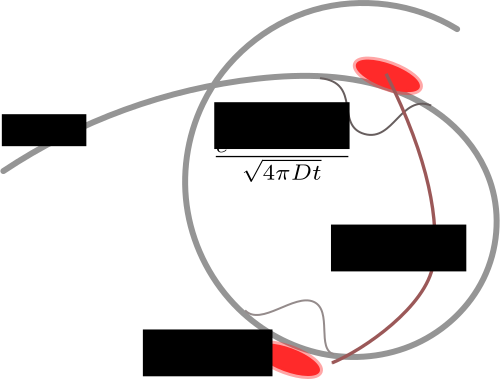
\includegraphics[width=0.7\textwidth]{TF_search.pdf}
% 	\caption{Illustration of combined 1D/3D search.}
% 	\label{fig:TF_search}
% \end{figure}

% \subsection*{Why is there an optimum?}
% One dimensional diffusion alone would be extremely inefficient since it takes very long time to scan the entire genome due to the square-root scaling of the distance covered.
% Very short $\tau_{1D}$, on the other hand, corresponds to very limited scanning of bases and in the limit of $\tau_{1D}\to 0$ corresponds to pure 3D search.
% Hence it is plausible that an optimum should exist.


Above, we have discussed models of cell-autonomous gene expression.
In the developing embryo, cells that are initially identical assume different fates and these fate decision are driven by the differential expression of genes.
The gene expression programs are controlled in space and time through the diffusion of signaling molecules or transcription factors and mechanical coupling of different parts of the embryo.
A paradigmatic example of spatial gene regulation through spatially spreading transcription factors is the activation of the gene \emph{hunchback} in the early Drosophila embryo.
For a short introduction into early Drosophila development, have a look at \url{https://youtu.be/Ncxs21KEj0g}.

\begin{figure}[tb]
	\centering
	\includegraphics[width=0.3\textwidth]{figures/Fluorescent_labeling_of_Bicoid_GFP_and_mRNA.jpg}
	\includegraphics[width=0.68\textwidth]{figures/fly_embryo.png}
	\caption{Left: Bicoid gradient (top) and RNA localisation (in red) in the lower panel (by Thomas Gregor, Julien O. Dubuis, Shawn C. Little).
	Right: Computational synthesis of gene expression patters in the fly embryo (from \url{https://dav.lbl.gov/archive/Events/SC05/Drosophilia/index.html}).
	}
	\label{fig:fly_gene_expression}
\end{figure}

Fig.~\ref{fig:fly_gene_expression} shows the earliest pattern -- the bicoid gradient --  on the left and a later more elaborate pattern of gene expression on the right.
As an example, we want to discuss the generation of the bicoid gradient and the resulting of {\it hunchback}.
The gene {\it hunchback} is expressed in the half of the cell with higher bicoid concentration with a very sharp boundary between cells that express it at full strength and those that don't: cells ``read'' the bicoid concentration and depending on whether this concentration is larger than a threshold, they express the target.
We will ask two questions: How is such a gradient established? And how is it read out?


\subsection*{Gradient formation by diffusion and decay}
Bicoid is produced at one end of the embryo through translation of mRNA that was deposited there by the mother.
The protein diffuses away from that pole through embryo.
That alone would slowly result in a homogeneous concentration of bicoid.
Bicoid, however, is unstable and degradation of bicoid coupled with diffusion results in a gradient.

For the purposes of studying the gene expression gradient, we only need to consider the long axis of the embryo, that it is sufficient to model the bicoid profile in one dimension.
Analogously to our discussion in chapter two (Eq.~\ref{eq:discrete_update}), we begin with a discrete one-dimensional model with spatial bins of width $\Delta x$, see Fig.~\ref{fig:reaction_diffusion}.
The concentration $b_i$ of bicoid in bin $i$ changes according to
\begin{equation}
	b_i(t+dt) = \delta_{i0}\alpha dt + (1-\beta dt )b_i + dt\frac{D}{\Delta x^2} (b_{i-1} - 2b_i + b_{i+1})
\end{equation}
Here $\beta dt$ is the fraction of bicoid that decays in a time interval $dt$, $\delta_{i0}\alpha dt$ is the production of bicoid that only happens in bin $i=0$, and the last term describes the discretized diffusion.
In analogy to Eq.~\ref{eq:diffusion}, this discrete equation is rewritten as a differential equation
\begin{equation}
	\frac{\partial b(x,t)}{\partial t} = \delta(x)\alpha + D\frac{\partial^2 b(x,t)}{\partial x^2} - \beta b(x,t)
\end{equation}
The ``delta-function'' $\delta(x)$ is a spike at $x=0$ and vanishes everywhere else.
This term models the production of bicoid at the very left end of the embryo.
The second term is the familiar diffusion term, while the last term models the degradation of bicoid with rate $\beta$.

We are interested in a steady state solution for $b(x,t)$ and we will first solve this equation for $x>0$ where the production term is absent.
Setting $\frac{\partial b(x,t)}{\partial t}=0$, we have for $x>0$
\begin{equation}
b(x) = \frac{D}{\beta}\frac{\partial^2 b(x)}{\partial x^2}
\end{equation}
This equation has the solution $b(x) = a e^{-\sqrt{\frac{\beta}{D}}x}$, i.e., the steady state concentration profile is an exponential decay with length scale $\ell = \sqrt{D/\beta}$.
The decay rate $\beta$ is the inverse of the bicoid life time $\tau = 1/\beta$ and the decay length can hence be rewritten as $\ell = \sqrt{D \tau}$.
The distance over which bicoid spreads from its source is hence given by a trade-off between diffusion and decay: The longer the protein lives, the shallower is the gradient.
And the scaling makes sense: after a typical lifetime $\tau$, we expect the bicoid to have moved a net distance of about $\sqrt{D\tau}$.

We can account for the production term by imposing a flux $\alpha$ through the boundary at $x=0$.
The flux is $-D\frac{\partial b(x)}{\partial x}|_{x=0}=a \sqrt{D\beta}=\alpha$ and therefore $a = \alpha/\sqrt{D\beta}$.
The full steady state solution is therefore
\begin{equation}
 	b(x) = \alpha \sqrt{\frac{\tau}{D}} e^{-x/\sqrt{D\tau}}
\end{equation}
Numerical solution of the discrete system agrees well with this analytical steady state solution, see Fig.~\ref{fig:reaction_diffusion}B.

\begin{figure}[tb]
	\centering
	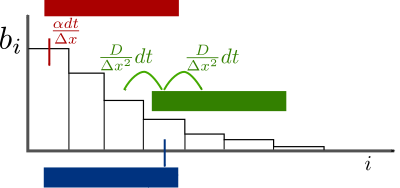
\includegraphics[width=0.48\textwidth]{reaction_diffusion.pdf}
	\includegraphics[width=0.48\textwidth]{figures/bicoid_gradient.pdf}
	\caption{Left: Discrete model of the reaction diffusion system governing the bicoid gradient.
	Right: Numerical solution of the discrete reaction diffusion equation and the analytical steady state solution.}
	\label{fig:reaction_diffusion}
\end{figure}

In a developing fly embryo, it seems that diffusion of bicoid is not simply a random walk of the molecule, but facilitated by large-scale back and forth movements of the cytosol during successive cycles of cell division.
For an overview of recent research on that topic, have a look at the online presentation by Eric Wieschaus at \href{https://youtu.be/cpOf5el9GIk}{youtu.be/cpOf5el9GIk}.

Careful fluorescence microscopy measurements of GFP-tagged Bicoid have shown that the gradient builds up over a scale of 2 hours and is extremely reproducible from one embryo to the next, see Fig.~\ref{fig:bicoid_gradient}.
This reproducibility is important to ensure the accurate separation of the embryo into anterior and posterior half.
This behavior can be quantitatively described by the reaction diffusion model discussed above.

\begin{figure}[tb]
	\centering
	\includegraphics[width=0.43\textwidth]{figures/Gregor_Bcd_gradient_buildup.png}
	\includegraphics[width=0.55\textwidth]{figures/Gregor_Bcd_gradient_reproducibility.png}
	\caption{Experimental characterization of the Bicoid gradient: Left) The gradient establishes itself over a time span of about 2 hours. Right: Different embryos have very similar Bicoid gradients at nuclear cycle 14. From \citep{gregor_stability_2007} and \citep{gregor_probing_2007}.}
	\label{fig:bicoid_gradient}
\end{figure}


\section{Patterning with reaction diffusion systems}
Reaction diffusion systems can generate much more interesting patterns than the gradient discussed above.
If two or more diffusion species interact, the result could be stationary patterns with spots or strips as well as dynamic wave-like patterns.
Many biological patterns (Zebra strips, leopard dots, etc) are believed to have their origin in such systems.
The best known such patters are {\it Turing patterns}.
\href{https://en.wikipedia.org/wiki/Alan_Turing}{Alan Turing} was a British mathematician who made many seminal contributions to computer science.
In addition, he showed that two-species reaction diffusion systems naturally generate many patterns common in biology \citep{turing_chemical_1952}.
These system have the general form
\begin{eqnarray}
	\frac{\partial u(x,t)}{\partial t} &=& D_u \frac{\partial^2 u(x,t)}{\partial x^2} + f(u(x,t),v(x,t)) \\
	\frac{\partial v(x,t)}{\partial t} &=& D_v \frac{\partial^2 v(x,t)}{\partial x^2} + g(u(x,t),v(x,t))
\end{eqnarray}
Often these systems are formulated in two dimensions, were they generate 6 distinct possible behaviors depending on the parameters and how the two species interact.
One class of these solutions forms stable patterns that often look very similar to patterns that one observes across the animal kingdom \citep{kondo_reaction-diffusion_2010}.

The basic mechanism of Turing patterns is often summarized as {\it short-range activation -- long-range inhibition}.
Both substances inhibit each others production and enhance their own production.
By tuning the ratios of diffusion constants, different types of patterns can be generated.

\begin{figure}[tb]
	\centering
	\includegraphics[width=0.98\textwidth]{figures/Kondo_Turing_patterns.png}
	\caption{Turing patterns. A) The generic states of a homogeneous reaction-diffusion system. B) Case V corresponds to traveling waves that often form spirals. The classical Turing patterns (Case VI) consist of stripes, dots, and domains for different parameters.
	C) These patterns are often very reminiscent of patterns observed in biology.
	From \citep{kondo_reaction-diffusion_2010}.}
	\label{fig:turing}
\end{figure}



% liquid-liquid phase transitions
 %!TEX root = main.tex
\chapter{Membraneless organelles and liquid-liquid phase transitions}


Major organelles in cells, e.g.~the nucleus, the ER, or mitochondria, are enclosed by membranes.
Transport between compartments is controlled by pores and channels.
This is not true for all organelles: structures like nucleoli and similar blobs in the cytosol seem to be well defined three dimensional structures without an enclosing membrane.
Over that last ten years, scientists have started to characterize such structures and discovered that these structures are essentially \emph{droplets} of one liquid embedded in another liquid (the cytosol) \citet{brangwynne_germline_2009}.

Among the earliest known examples of membraneless organelles are nucleoli can Cajal bodies.
Nucleoli were first described in the early 19th century.
Subsequently, it was shown that nucleoli are the structures in which ribosomal RNAs are transcribed.
They form seemingly homogeneous structures with a markedly different protein and RNA composition than the surrounding nucleus without being enclosed by a membrane.
Cajal bodies were first described by Santiago Ramon y Cajal.
They are often associated with nucleoli and seem to be involved in various steps of RNA processing.
There exact function is not well described.

Cytosolic membraneless structures include stress granules, P-bodies, or P-granules.
These granules form in particular developmental stages or specific environmental conditions.
Most fundamental discoveries about the nature of such membraneless organelles have been made with P-granules which are important in early C.~elegans development.
P-granule stands for ``perinuclear RNA-rich cytoplasmic granule''.
They are mixtures of RNA and RNA-binding-proteins many of which are implicated in translational control (possibly due to their P-granule association.)
In their seminal paper, \citet{brangwynne_germline_2009} show that these P-granules behave like liquid droplets immersed in the cytosol and that condensation and dissolution of these droplets are governed by physical principles of phase transitions.
Biology seems to exploit these principles to achieve an efficient separation of protein and mRNA between two daughter cells of the first cell division in C.~elegans development.
Such liquid-liquid phases transitions have since been discovered in many cell biological contexts.
While their precise role often remains elusive, it by now seems clear that such condensates and phase transitions are an important facet of organization in cells.


\section{Phase transitions}
Phases and phase transitions are part of our day-to-day experiences: water freezes and boils, oil and water don't mix, eggs become hard as you boil them.
Fig.~\ref{fig:h2o_phases} shows a simplified phase diagram of water with the solid (ice), liquid (water), and gaseous (vapor) phases.

The part of the phase diagram that will be of greatest interest here is the boundary between the liquid and the vapor phase.
This boundary has a sudden end in a critical point.
Have a look at the video \href{https://youtu.be/-AXJISFdC2E}{youtu.be/-AXJISFdC2E}, which shows the behavior of a substance in the vicinity of the critical point.
Below the critical point, the system can coexist in two phases.
As one approaches the critical point, the density of gas and vapor become more similar until at the critical point the differences between the two phases disappears.
Above the critical point, the substance is homogeneous -- a state known in super-critical liquid.

The aspect of the phase diagram that is most relevant for our discussion below in that of condensation: Consider a system in the vapor phase. As you begin to cool down the system, vapor at some point becomes super-saturated and it condenses into droplets (fog).
This condensation corresponds to approaching the boundary between the liquid phase and vapor phase horizontally.

\begin{figure}[tb]
	\centering
	\includegraphics[width=0.8\textwidth]{figures/Phase_diagram_of_water_simplified.png}
	\caption{Simplified phase diagram of water as a function of temperature and pressure. Ambient pressure is indicated by a horizontal line, 0$^\circ$C and $100^{\circ}$C are indicated by horizontal lines.}
	\label{fig:h2o_phases}
\end{figure}


\subsection*{Phases of multicomponent systems}
The discussion above used water as an example.
Water has a rich phase diagram, but this example has one fundamental limitation: nothing else but $\mathrm{H_2 O}$.
All systems we will encounter in biology are complicated mixtures of many different types of molecules that can interact in myriad ways.
From thermodynamics, you should be familiar with Gibb's phase rule:
\begin{equation}
	f = c - p + 2
\end{equation}
Here, $f$ is the number of degrees of freedom, $c$ is the number of components, and $p$ is the number of co-existing phases.
It immediately follows that systems composed of many different molecular species ($c$) can co-exist in many different phases $p$.
At co-existence, these phases share the same temperature and pressure, but differ in composition of the different species.
The relative amount of each phase and its composition adjusts such that the chemical potential of each compound is equal in each phase.
These compositions can either be almost completely pure species (like oil and water mixtures) or more even mixtures (like 30/70).
The closer the system is to a critical point, the more even the mixtures are.
Whether a multi-component system separates into several phases depends not only on the temperature, pressure and the composition of the system.


\section{Multi-component systems}

\subsection*{Entropy and energy mixtures}
The phase separation, or de-mixing, is driven by conflicting entropy and energetic (enthalpic) tendencies.
The energy of the system is minimized by placing molecules that interact  favorably with each other next to each other.
Entropy, on the other hand, is maximized by randomly distributing the species in space resulting in one homogeneous phase.
We will now explore these competing tendencies in a simple toy model of a solution of a self-interacting species in a solvent, see Fig.~\ref{fig:multi_component_mixtures}.

\begin{figure}[tb]
	\centering
	\includegraphics[width=0.7\textwidth]{figures/Brangwynne_interactions.png}
	\caption{Illustration of multi-component mixtures. From \citet{brangwynne_polymer_2015}.}
	\label{fig:multi_component_mixtures}
\end{figure}

The white balls in Fig.~\ref{fig:multi_component_mixtures} represent the solvent, the green balls the protein or polymer whose condensation we are interested in (we'll call it protein for simplicity).
The interaction energy can be written as the number of contacts between solvent molecules $u_{ss}$, between solvent and protein $u_{sp}$, and between proteins $u_{pp}$.
The total energy of the mixture is therefore given by
\begin{equation}
	U = n_{ss}u_{ss} + n_{sp}u_{sp} + n_{pp}u_{pp}
\end{equation}
where $n_{ss}$, $n_{sp}$, and $n_{pp}$ are the number of times the respective neighbor relations are observed.

While we will never be able to enumerate the exact number of neighbor relations, we can readily estimate the expected number of contacts.
The typical number of contacts one solvent molecule makes is called the coordination number $z$.
For simplicity, lets assume that monomers have similar size as solvent molecules and arrange them on a lattice.
If the state of the systems is a random mix with monomer fraction $\phi$, the energy of the system is
\begin{equation}
\begin{split}
U &= \frac{N z}{2} \left[(1-\phi)^2 u_{ss} + \phi^2 u_{pp} + 2\phi(1-\phi)u_{sp}\right] \\
&= \frac{N z}{2}\left[\phi(1-\phi)(2u_{sp} - u_{pp}-u_{ss}) + \phi(u_{pp}-u_{ss}) + u_{ss}\right]
\end{split}
\end{equation}
The term proportional to $\phi(1-\phi)$ is the contribution of contacts between the types, while the term proportional to $\phi$ is simple the difference between the pure types.
The take home here is that as a function of concentration $\phi$, the enthalpy is a parabola that can either have positive curvature favoring mixtures or negative curvature favoring demixing.

Demixing is opposed by entropy: many energetically unfavorable states can have more weight than few favorable states.
Entropy is the logarithm of the number states available given the constraints.
Consider a lattice model of the solution and ignore for a moment that the monomers of the polymer are strung together.
In a random mixture, we can pick for each lattice site independently whether its solvent or monomer.
This results in
\begin{equation}
e^{(S+c)/k} = \frac{N!}{(N\phi)!(N(1-\phi))!}
\end{equation}
configurations (where $k$ is Boltzmann's constant).
The logarithm of this number is the entropy (up to an additive constant).
To calculate its magnitude, we use the well known Stirling's approximation for factorials $\log n! \approx n\log n - n$ and find
\begin{equation}
\begin{split}
S + c &= kN\left[\log N - \phi\log(\phi N) - (1-\phi)\log((1-\phi)N)\right] \\
& = -N(\phi\log(\phi) + (1-\phi)\log(1-\phi))
\end{split}
\end{equation}
Combining the interaction energy with the mixing entropy, we arrive at the free energy $F=U-TS$ of the idealized system (assuming $u_{pp}=u_{ss}$ and dropping constants):
\begin{equation}
\frac{F}{N} =  \phi(1-\phi) \frac{z(2u_{sp} - u_{pp}-u_{ss})}{2} + kT\left[\phi\log(\phi) + (1-\phi)\log(1-\phi)\right]
\end{equation}
Whether the solution will spontaneously separate into a phase of high and low concentration of the protein, depends on whether the free energy of the homogeneous mixed system is lower than the sum of the energies of two systems at high/low monomer concentration.


\subsection*{Instability of a mixture}
Consider a homogeneous mixture with monomer concentration $\phi$ and compare this to a two phase mixture in which one phase (fraction $\alpha$) has concentration $\phi_1$ and the other phase (fraction $1-\alpha$) has concentration $\phi_2$.
To conserve mass $\alpha \phi_1 + (1-\alpha)\phi_2 = \phi$.
Under what conditions will a mixture of two phases will have lower energy than the homogeneous case?

The stability of a configuration depends on the curvature of the free energy in $\phi$.
This is illustrated in Fig.~\ref{fig:unstable_mix}.
The free energy of a mixture with fraction $\alpha$ lies on a straight line connecting the two pure phases with concentrations $\phi_{1/2}$.
Conservation of mass requires that the average concentration doesn't change, hence the relevant comparisons are all on a vertical line.
This considerations immediately tells us that a mixture is stable if the free energy is convex, i.e., the curvature is positive.
Otherwise, it is always possible to lower the free energy by splitting the solution into a mix of two phases.

\begin{figure}[tb]
	\centering
	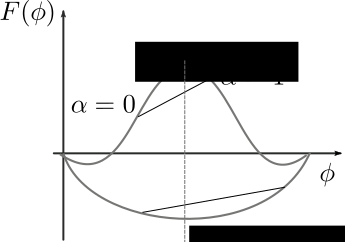
\includegraphics[width=0.6\textwidth]{unstable_mix.png}
	\caption{Unstable mixture}
	\label{fig:unstable_mix}
\end{figure}

\subsection*{Surface tension}
Phase separation happens when like interactions are sufficiently strong to overcome entropy favoring mixing.
At the surfaces of two phases, however, molecules enjoy a smaller number of like interactions than in the bulk of the either phase.
Hence surfaces between phases are associated with a free energy cost.
This cost results in a tendency to minimize the surface area given the volume and the optimal geometry is obviously a sphere.
Effectively, the surface is under tension driving shapes towards the lowest free energy geometry.
Surface tension has units energy/area or Newton/length.

When three different phases (or a solid, a liquid and a gas) meet, the three phase interface depends on the relative surface tensions associated with the three interfaces.
The resulting behavior and contact angles can be calculated from the balance of forces at the contact line.

\subsection*{Nucleation}
A homogeneous solution can get super-saturated.
Super-saturation refers to a state where the system should have separated into two phases, but this separation hasn't happened yet.
Such delayed condensation can occur since the forming small droplets can be energetically disfavorable even though the equilibrium state would favor phase separation.
This phenomenon is known from our atmosphere: It is possible to ``seed'' clouds with small particles to produce rain.
These small particles act as nuclei around which rain drops can form -- a process energetically more favorably than drop formation without a nucleus.

The energetic barrier for nucleating a droplet can be understood by a simple argument involving the scaling of the surface and the bulk of a droplet.
The relative contributions of free energy of the bulk and surface depend on the size of the droplet.
For a spherical droplet, the free energy will scale with the radius as
\begin{equation}
G(r) = -\alpha r^3 + \beta r^2
\end{equation}
where $\alpha,\beta$ are positive constant with the appropriate dimensions.
At very small $r$, the free energy increases with $r$ and small droplets are unstable.
Only above the nucleation radius $r^* = \frac{2\beta}{3\alpha}$ do droplets grow deterministically.
This phenomenon is known as nucleation.
One common every day example were nucleation can be observed is the instant freezing of super-cooled water.
Have a look at this video \href{https://youtu.be/PM9nwYF1uR4}{youtu.be/PM9nwYF1uR4}.


\section{Condensates in biology}

\subsection*{Droplets are often RNA-protein mixtures}
To drive phase separation and form droplets, the constituents need to be able to form multivalent interactions.
Obviously, 1-1 interactions can't form higher order structures, only dimers.
Similarly, if each molecule can only interact with two other molecules, one can form polymer chains by no extended 3D structures.
Instead, at least 3-valent at better still multi-valent interactions are necessary to drive phase transitions.
In the lattice example above, the multi-valency was given by the number of neighbors on the lattice.
In droplets in the cytosol, such multivalent interactions are mediated by intrinsically disordered regions of proteins that often contain repetitive linear motives that interact with each other or RNA.
These regions are also called low complexity regions due to their repetitive sequence and biased amino acid composition.
Fig.~\ref{fig:mol_interactions} shows several such low complexity regions in different proteins along with the types of interactions they generate.

\begin{figure}[tb]
	\centering
	\includegraphics[width=\textwidth]{figures/Brangwynne_molecular_basis.png}
	\caption{Modes of multivalent interactions in different types of cytosolic droplets. Figure from \citet{brangwynne_polymer_2015}.}
	\label{fig:mol_interactions}
\end{figure}

Similarly, interactions between RNA and proteins can generate droplets: RNA can serve as a scaffold that is cross-linked many times by proteins (or protein complexes) that have at least 2 RNA binding domains.

\subsection*{P granules in {\it C.~elegans}}
The notion that membraneless organelles might be essentially liquid droplets embedded in the cytosol was put forward in a publication in 2009 by \citet{brangwynne_germline_2009}.
P-granules are protein-RNA assemblies that are involved in the determination of cell fate in the early {\it C.~elegans} embryo, see Fig.~\ref{fig:pgranules}.
Initially, P-granules are distributed across the embryo and appear and dissolve in a spatially homogeneous fashion.
They move around by cytoplasmic flow.
This flow does in fact transport as many P-granules left as it does right.
Nevertheless, P-granules concentrate at the posterior end.
This concentration is caused by different conditions in the anterior and posterior ends: Droplets dissolve at the anterior end and form at the posterior end.
This effectively introduces a sink which concentrates the droplets in one of the daughter cells.

\begin{figure}[tb]
	\centering
	\includegraphics[width=\textwidth]{figures/Brangwynne_Pgranules_intro.png}
	\caption{P-granules in {\it C.~elegans} embryos. Figure from \citep{brangwynne_germline_2009}.}
	\label{fig:pgranules}
\end{figure}

These droplets are remarkably dynamic.
Photobleaching of fluorescently labeled droplet components shows that components rapidly diffuse across the droplet and also move between the cytosol and the droplet.
When sheared, P-granules flow, drip, and wet just like liquids.


\begin{figure}[tb]
	\centering
	\includegraphics[width=\textwidth]{figures/Brangwynne_Pgranules_liquid.png}
	\caption{P-granules behave like liquids that rapidly exchange material with the surrounding cytosol. Figure from \citep{brangwynne_germline_2009}.}
	\label{fig:pgranules_liquid}
\end{figure}

\subsection*{Putative functional roles of condensates}
The function of membraneless organelles continues to be poorly characterized, but several plausible hypotheses exist:
\begin{itemize}
	\item {\it micro-reactors}: Droplets are greatly enriched for particular sets of proteins and RNAs. Hence specific reactions between these components are expected to be much faster in such droplets compared their speed if components were randomly distributed in the cytosol.
	\item {\it garbage dumps}: uncontrolled protein aggregation is dangerous. Hence droplets could represent a controlled way to absorb excess material that would otherwise be prone to uncontrolled aggregation. Similar, the droplets could serve to sequester harmful (damaged, misfolded, etc) proteins.
	\item {\it storage:} Membraneless organelles could be used for RNA storage that would be ready for transcription and/or modification when the conditions change.
\end{itemize}
As more research is done, the roles of droplets will become better defined and more roles will likely be discovered.
Compartmentalization plays an important role at many scales of biological organization and there is every reason to believe that biology exploits the potential of membraneless organelles.

% Polymers
%!TEX root = main.tex
\chapter{Polymers}

Many of the most important molecules in biology are polymers:
DNA and RNA encode genetic information in the order of bases, proteins are polypeptides, and the cytoskeleton provides structure and stability to cells.
We will discuss properties of
\begin{itemize}
	\item single stranded RNA and DNA
	\item double stranded DNA
	\item cyctoskeletal filaments
\end{itemize}
The microscopic properties of these different polymers depend on their molecular structure, but on larger scales their behavior is governed by a few mesoscopic parameters such as stiffness, charge, self-interaction, and cross-linking.
These large scale properties can be studied with abstract models.
Polymers are also ubiquitous in our every day life: rubber, plastics, many textiles, and many food items are made from polymers.
These materials have often surprising properties which can be understood with mathematical models.
The physical properties of polymers are dictated by a trade-off between entropy and energy: Bending a polymer typically requires energy, but there are many more bent and coiled confirmations than straight confirmations.
Depending on how this trade-off plays out, we expect these polymer configurations to vary from straight rods to messy coils.


\begin{figure}[tb]
	\centering
	\includegraphics[width=0.44\textwidth]{lysed_ecoli.jpg}
	\includegraphics[width=0.55\textwidth]{figures/cytosceleton_RGB.png}
	\caption{Left: DNA from a lysed E coli (source: http://i.imgur.com/kaFF3.jpg) reveals its long filamentous structure. Right: The cytosceleton provides structure and rigity to the cell. Actin filaments are shown in green, tubulin in blue, DNA in red.}
	\label{fig:polymer_overview}
\end{figure}

\section{Polymers as information carriers}
DNA and RNA are hetero-polymers -- long chains of similar but not identical subunits.
These subunits are covalently strung together and their order encodes information -- much like letters in a text.
To full-fill their function, these polymers need to be
\begin{itemize}
	\item sufficiently stable
	\item accessible
	\item allow for accurate synthesis and copying
\end{itemize}
These requirements are more severe for DNA than for mRNA, which serves mostly as an intermediate message.

\section{Proteins are polymers}
Proteins are folded polypeptide chains (hetero-polymers as above).
But instead of storing or transmitting information, the order of amino acids in the polypeptide determines the fold and function of the protein.
The linear order of the amino acids is not crucial for the final product, but likely essential in the folding process: detached amino acids in solution would never assemble into a globular protein.
Protein folding and denaturation was covered at great length by Sebastian Hiller and we won't discuss this again here.

\section{Polymers as structural elements}
The aspects of polymer that we'll study in most detail here is how cells use them to exert force and control shape.
The three main classes of filaments of the cytoskeleton are
\begin{itemize}
	\item actin filaments
	\item microtubuli
	\item intermediate filaments
\end{itemize}
Actin and microtubuli are made from small globular proteins that associate non-covalently to form long filaments.
Intermediate filaments are made from ``coiled-coil'' subunits that make them exceptionally extendable.

These different filaments have very different mechanical properties.
These properties can -- to a large extent -- be understood using physical reasoning on how monomers assemble into filaments, how long they are, and how filaments are cross-linked to each other.

\begin{figure}[tb]
	\centering
	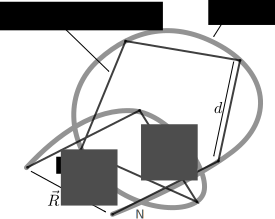
\includegraphics[width=0.43\textwidth]{figures/jointed_chain.pdf}
	\includegraphics[width=0.55\textwidth]{figures/Genome_conformation_van_den_Engh.png}
	\caption{Illustration of the simple discrete polymer models.
	Right: Mean squared separation of chromosomal markers as a function of their genomic distance. Data from \citet{engh_estimating_1992}.}
	\label{fig:polymer_models}
\end{figure}

\section{The freely jointed chain model}
In the micrograph in Fig.~\ref{fig:polymer_overview}, it is obvious that DNA often changes direction in a seemingly random way.
One of the simplest models of such a polymer is the \emph{jointed chain} model.
As illustrated in Fig.~\ref{fig:polymer_models}, this model replaces the polymer by a chain of stiff elements of length $d$.
At each joint, the direction of the polymer can change.
If it changes very little the polymer is stiff and will change direction only slightly, if these direction changes are more drastic, the polymer ends of being a random coil.
Using such models, we can answer questions like (i) how far apart from each other is the beginning and the end-point of the chain, or (ii) how much space does the polymer coil occupy?

The simplest models of polymers -- the freely jointed chain model -- assumes that the direction randomizes completely at each joint.
Consider a chain of $N$ stiff segments of length $d$.
Within the freely jointed chain model, the end-to-end distance of the chain is
\begin{equation}
	\vec{R} = d \sum_{i=1}^N \vec{e}_i
\end{equation}
where $\vec{e}_i$ is a vector of length 1 pointing in the direction of the segment $i$.
Since this direction is chosen completely at random, this model is essentially a random walk in three dimensions.
The average end-to-end vector is hence zero since the endpoint is equally likely to end up on the left, right, above, below, before, or behind the starting point.
This situation is analogous to diffusion or random walks.
To get a meaningful sense of the separation of the end points, we need to calculate the mean squared end-to-end distance:
\begin{equation}
\begin{split}
\label{eq:FJC}
	\langle \vec{R}^2 \rangle &= d^2\langle\sum_{i}^N \vec{e}_i\sum_{i}^N \vec{e}_j\rangle = d^2\sum_{i,j=1}^N \langle\vec{e}_i\vec{e}_j\rangle \\
	& = d^2\sum_{i=1}^N \langle \vec{e}_i^2 \rangle + d^2\sum_{i,j=1, i\neq j}^N \langle \vec{e}_i\vec{e}_j \rangle = d^2N
\end{split}
\end{equation}
In the last step, we split the sum over $i$ and $j$ into two sums: the first sum contains all terms where $i=j$, the second one only contains the terms where $i$ and $j$ differ.
The first sum evaluates to $d^2N$ since each term $\vec{e}_i^2=1$.
This second sum is simply 0 since the direction of segment $i$ is completely independent of segment $j$.
The typical end-to-end separation therefore grows with the length of the polymer as $\sqrt{\langle \vec{R}^2 \rangle} = d\sqrt{N}$.
This result is familiar from our study of random walks and diffusion.
In addition to the squared end-to-end distance, polymers are often characterized by the radius of gyration defined as
\begin{equation}
	R_g^2 = \frac{1}{N}\sum_{i=1}^N (\vec{r}_i - \vec{R}_{cm})^2 = \frac{d^2N}{6}
\end{equation}
where $\vec{r}_i$ is the position of monomer $i$ and $\vec{R}_{cm}$ is the center of mass.
The radius of gyration is essentially the width of the polymer coil and its scaling properties are the same as the end-to-end distance.

Despite the simplicity of this model, the basic dependence of the end-to-end distance on the length of the polymer is observed in biology.
\citet{engh_estimating_1992} measured the distance between two position on the human chromosome 4 labeled with fluorescent probes.
These measurements were repeated for many pairs of positions varying between $10^5$ and $4\times 10^6$ base pairs, see Fig.~\ref{fig:polymer_models}.
When plotting the mean-squared marker-to-marker distance against they separation on the chromosome, \citet{engh_estimating_1992} observed a linear relationship consistent with Eq.~\ref{eq:FJC}.

The linear relationship not only confirm the basic properties of the model, it allows us to estimate the length after which the direction of the genome is effectively randomized.
To do so, we use following
\begin{itemize}
	\item The chromosomal distance between markers can be expressed in multiples of the unknown segment length $d$ as $x = nd$.
	\item The average squared distance of the markers in 3D is expected to be $\langle \vec{R}_n^2\rangle = nd^2$.
	\item According to Engh et al, $\langle \vec{R}_n^2\rangle = \alpha x$.
\end{itemize}
Substituting these relationships into each other, we find
\begin{equation}
	\langle \vec{R}_n^2\rangle = nd^2 = \alpha x = \alpha n d \quad \Rightarrow \quad d=\alpha
\end{equation}
The slope $\alpha$ in the graph is about $2\times 10^{-6}\mu m^2/bp$.
Since one base pair in dsDNA is $0.34nm = 3.4\times 10^{-4}\mu m$, $\alpha = 6\times 10^{-3} \mu m$.
In a human cell, the DNA is wrapped around histones and the diameter of a histone is roughly comparable to length on which DNA randomizes its direction according to this simple model.


\subsection*{Polymer stiffness}
The freely jointed chain model is extremely simplistic: it models the polymer as a chain of completely stiff segments with freely rotating joints.
In reality, polymers are stiff and resist bending.
So why is that simple model a good starting point?

Real polymers changes direction mainly by two distinct modes: (i) rotation around a bond, or (ii) bending of a structure that resists rotation.
After several rotations or many slights bends, the direction randomized and the conformation of the polymer is effectively described by the simple model above.
We will investigate how the simple model emerges as an effective model using two different scenarios.


\subsubsection*{Freely rotating chains}
The freely rotating chain model assumes that adjacent monomers have an angle $\theta$, but can rotate freely rotate around the azimuth.
We can now repeat the calculation of the end-to-end distance in Eq.~\ref{eq:FJC}, but have to account for the fact that $\langle \vec{e}_i\vec{e}_j \rangle$ is no longer 0 for all $i\neq j$.
For neighboring monomers, the average over all possible rotation angles is obviously
\begin{equation}
	\langle \vec{e}_i\vec{e}_{i+1} \rangle = \cos \theta
\end{equation}
Now a correlation between vectors $\vec{e}_i$ and $\vec{e}_{i+2}$ can only be mediated by a monomer $i+1$ and with each intervening monomer the correlation drops by a factor $\cos \theta$.
We thus have
\begin{equation}
	\langle \vec{e}_i\vec{e}_{j} \rangle = \left(\cos \theta\right)^{|j-i|} = \alpha^{|j-i|}
\end{equation}
The calculation of the end-to-end distance involves summing over the correlation between all pairs of monomers:
\begin{equation}
\begin{split}
\label{eq:FRC}
	\langle \vec{R}^2 \rangle &= d^2 N + 2d^2\sum_{i=1}^{N}\sum_{j=i+1}^N \langle \vec{e}_i\vec{e}_j \rangle  \\
	&  =d^2 N + 2d^2\sum_{i=1}^{N}\sum_{k=1}^{N-i} \alpha^k = d^2 \left(N + 2\alpha\sum_{i=1}^N \frac{1-\alpha^{N-i-1}}{1-\alpha}\right)
\end{split}
\end{equation}
If the chain is long ($N\gg1$), we can neglect $\alpha^{N-i}$ in the numerator and the expression simplifies to
\begin{equation}
\begin{split}
\label{eq:FRC_approx}
	\langle \vec{R}^2 \rangle &\approx d^2 N \left(1 + 2\frac{\alpha}{1-\alpha}\right) = d^2 N \frac{1+\cos\theta}{1-\cos \theta}
\end{split}
\end{equation}
This relation, together with the overall length of the polymer contour, allows us to calculate the an effective monomer length that maps the behavior of the Free Rotating Chain to the Freely Jointed Chain.
The backbone length is $L = dN \cos (\theta/2)$ (when stretched, the polymer will take a zig-zag-configuration where each element is at an angle $\theta/2$.)
If we now want to find a Freely Jointed Chain model with $M$ monomers of length $l_k$ that has the same contour length and average squared end-to-end distance, we need to fulfill the relations
\begin{equation}
	\begin{split}
		N d \cos (\theta/2) = M l_k \\
		N d^2  \frac{1+\cos\theta}{1-\cos \theta} = M l_k^2
	\end{split}
\end{equation}
This is readily solved by (substitute $M = (N d \cos(\theta/2))/l_k$ into the second equation)
\begin{equation}
	\begin{split}
		l_k = \frac{d}{\cos(\theta/2)} \frac{1+\cos\theta}{1-\cos \theta} \\
		M = N \cos(\theta/2)^2 \frac{1-\cos \theta}{1+\cos\theta}
	\end{split}
\end{equation}
This effective length $l_k$ is often called Kuhn length after the physical chemists Hans Kuhn and Werner Kuhn (who happened to have worked at the University of Basel and served as Rektor for several years) \citep{kuhn_uber_1934}.


\subsubsection*{Worm-like chain model}
In the above model, direction changed due to rotation around covalent bonds.
Such rotation is possible in single stranded nucleotide chains or peptides, but not in polymers like double stranded DNA or cytoskeletal polymers.
In these polymers, direction changes because of small bends that happen along backbone in analogy to bending of a beam or spaghetti.
At the molecular scale, this bending is due to thermal excitation and the persistence of a polymer will depend on the energy it takes to bend it compared to the thermal energy $kT$.
To bend a beam of length $L$ with stiffness $\kappa$ into an arc with curvature radius $R$, we require an energy $\kappa L/2R^2$.
To have the polymer change direction, it needs to be curved by a radius $\ell_p$ over a distance $\sim \ell_p$ and the required energy should be comparable to $kT$: $kT \approx \kappa /2\ell_p$.
A more careful calculation shows that the length scale over which the direction of the polymer decorrelates -- known as \emph{persistence length} -- is given by
\begin{equation}
	\ell_p  = \frac{\kappa}{kT}
\end{equation}
With this definition, the tangent-tangent correlation of two points on the polymer is $\langle \vec{e}(s)\vec{e}(t)\rangle = \exp(-|t-s|/\ell_p)$.
The Kuhn length of the worm-like chain model is $2\ell_p$.


\begin{figure}[tb]
	\centering
	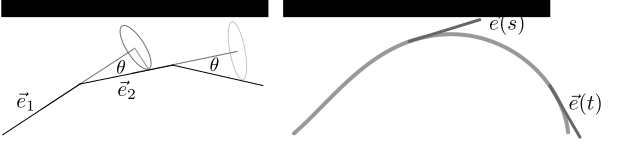
\includegraphics[width=0.96\columnwidth]{figures/stiff_polymers.pdf}
	\caption{{\bf Polymers with stiffness.} The freely rotating chain model (left) assumes that different monomers are at a fixed angle but can rotate freely around the bond. The worm-like chain model is more appropriate for polymer that bend only slightly at individual bonds and where directional changes are occur only after many monomers. The worm-like chain model is characterized by a persistence length that describes the decay in directional correlation between tangent vectors at different positions along the polymer. }
	\label{fig:stiff_polymers}
\end{figure}



\section*{Polymers under force}




\subsection*{Pulling -- optical tweezers}
The 2018 Nobel prize in physics was partly awarded to \href{https://en.wikipedia.org/wiki/Arthur_Ashkin}{Arthur Ashkin} for the development of optical tweezers -- a method to manipulate microscopic objects and measure forces on the pico-newton scale.
In this technique, a focused laser beam traps tiny particles in the center of the focus where the light intensity is highest.
Forces applied to these particle move the trapped particles slightly out of the focus of the beam and diffract light in a way that allows to measure the force applied, see Fig.~\ref{fig:DNA_stretching}.

\begin{figure}[tb]
	\centering
	\includegraphics[width=0.6\textwidth]{figures/OpticalTweezers_DNA.png}
	\includegraphics[width=0.39\textwidth]{figures/DNA_force_extension.png}
	\caption{Polymers under force. Left: Schematic representation of an optical tweezer (by \href{http://umdberg.pbworks.com/w/page/47555271}{Joe Redish}). Right: Force-extension curve of double stranded DNA from \cite{bustamante_entropic_1994}.
	The dashed line is the prediction by the freely jointed chain model, the solid line the prediction by the worm-like chain model.}
	\label{fig:DNA_stretching}
\end{figure}

When stretching a flexible polymer, the confirmation changes drastically:
Initially, the polymer is a random coil and the force merely displaces the two end points away from each other.
In this regime, the force generated by the polymer is of ``entropic'' nature.
At higher forces, the end-to-end extension approaches the contour length and the resistance to further extension stems from the elasticity.

\subsubsection*{Entropic springs}

Flexible polymers form random coils and the average end-to-end distance is typically proportional to the square root of the length of the chain.
What happens if you start to pull on the ends? Will it immediately stretch? Or will it act as a spring? How does extension depend on the applied force and the length of the spring?

Let's consider a polymer that consists of segments of length $d$ that are completely freely rotating, i.e., any angle on the sphere is equally likely a priori.
Applying a force will bias this distribution.
The probability of for any given monomer to have an extension $\chi$ is therefore
\begin{equation}
p(\chi|F) = \frac{F}{kT}\frac{e^{F\chi/kT}}{e^{Fd/kT}-e^{-Fd/kT}}
\end{equation}
(this has units $1/length$ as it should.)
The total end-to-end distance in the direction of the force is $x=\sum_i \chi_i$ and the average extension is simply
\begin{equation}
\begin{split}
\langle x \rangle_{F} &= N\int_{-d}^d d\chi \; \chi p(\chi|F) = \frac{FN}{kT(e^{Fd/kT}-e^{-Fd/kT})} \int_{-d}^{d} d\chi \;\chi e^{F\chi/kT} \\
% &= \frac{FN}{kT(e^{Fd/kT}-e^{-Fd/kT})} \int d\chi \; kT \frac{\partial }{\partial F} e^{F\chi/kT} \\
% &= \frac{FN}{e^{Fd/kT}-e^{-Fd/kT}} \frac{\partial }{\partial F}\frac{kT}{F} \left(e^{Fd/kT} - e^{-Fd/kT}\right) \\
% & = \frac{FN}{e^{Fd/kT}-e^{-Fd/kT}} \left(-\frac{kT}{F^2} + d\left(e^{Fd/kT} + e^{-Fd/kT}\right)\right)
& = dN \left(\frac{e^{Fd/kT}+e^{-Fd/kT}}{e^{Fd/kT}-e^{-Fd/kT}} - \frac{kT}{Fd}\right)
\end{split}
\end{equation}
Let's expand this around $F=0$:
\begin{equation}
\langle x \rangle_{F} \approx F\frac{\partial \langle x \rangle_{F}}{\partial F} =  F\frac{d^2N}{3kT}
\end{equation}
Hence to lowest order in $F$ a flexible polymer acts as an entropic spring with spring constant $\frac{3kT}{d^2N}$.
Longer polymers are softer, and increasing temperature makes them stiffer. The smaller the monomers are, the stiffer they are.
This is a well known effect in rubber bands.
Rubber bands are effectively many tightly entangled and cross-linked polymers.
When heated, the flexible bits undergo more vigorous thermal motion resulting in a stronger force resisting extension.
You can find various demonstrations of this effect online, for example \href{https://www.youtube.com/watch?v=eB4B2xZI77A}{in this video}.

\begin{figure}[tb]
	\centering
	\includegraphics[width=0.35\textwidth]{figures/Microtubule_structure.jpg}
	\includegraphics[width=0.62\textwidth]{figures/actin_filament.png}
	\caption{Left: Structure of microtubules. Right: 13 subunit structure of actin filament. Both graphs  are by Thomas Splettstoesser (www.scistyle.com) and retrieved from wikipedia)}
	\label{fig:cytoskeleton_structure}
\end{figure}

A typical RNA molecule with $N=1000$ and $d=2nm$, we would find a spring constant
\begin{equation}
\alpha = \frac{3kT}{d^2N} = \frac{12pN nm}{4nm^2 1000} = 3\times 10^{-3}\frac{pN}{nm}
\end{equation}

In the opposite limit around $x=d$, the behavior of the force extension curve is very different.
\begin{equation}
\langle x \rangle_{F} \approx Nd\left(1 - 2e^{-\frac{Fd}{kT}} + \cdots - \frac{kT}{Fd}\right) \approx Nd\left(1 - \frac{kT}{Fd}\right)
\end{equation}
This implies that at large force $Fd\gg kT$ the polymer is almost completely extended.
Solving this relation for the force yields
\begin{equation}
F = \frac{kT}{d(1- \langle x \rangle/Nd)}
\end{equation}
Hence the force diverges as the polymer approaches full extension.

\begin{figure}[tb]
	\centering
	\includegraphics[width=0.5\textwidth]{figures/Brangwynne_microtubule_buckling.jpg}
	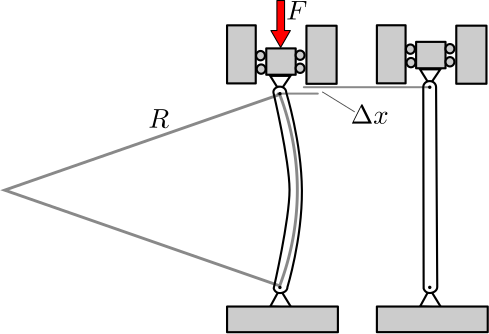
\includegraphics[width=0.48\textwidth]{figures/buckling.pdf}
	\caption{Polymers under force: Buckling of microtubules in cells \citep{brangwynne_microtubules_2006}.}
	\label{fig:buckling}
\end{figure}

\subsection*{Pushing -- buckling instabilities }
If you compress the ends of an elastic rod, it will resist the force until at some point it starts to collapse rapidly.
This is called \emph{buckling}.

How much compressive force can microtubules or other biopolymers withstand before they start to buckle?
Let's write down the energy of a rod of length $L$ when a force $F$ is applied.
When the rod bends, its end-to-end distance gets shorter and the energy of the system is changes do the displacement in the direction of the force (reduction in energy) and the bending of the rod.
The curvature is commonly described by the radius $R$ of the circle that overlaps with the rod's contour.
We will approximate the contour of the rod by an arc of a circle and assume bending is slight, that is the curvature radius $R$ is much bigger than the contour length $L$.
The angle of the arc is $\theta = L/R$ and the end-to-end distance is
\begin{equation}
 x = 2R\sin(L/2R) \approx L - \frac{L^3}{24R^2}
\end{equation}
The displacement in the direction of the force is hence $L^3/24R^2$ and the total energy is
\begin{equation}
E_{tot} = E_{bend} + E_{load} = \frac{\kappa L}{2R^2} + FL(1 - \frac{L^2}{24R^2})
\end{equation}
With increasing curvature (decreasing $R$), the first term increases and the second term decreases.
Whether the total energy increases or decreases depends on the force and parameters of the rod.
We can rewrite the total energy as
\begin{equation}
	E_{tot} = FL + \frac{L}{2R^2}\left[\kappa -\frac{FL^2}{12}\right]
\end{equation}
This tells us that as soon as the force exceeds
\begin{equation}
F_c \approx \frac{12\kappa}{L^2}
\end{equation}
increasing the curvature will further reduce the total energy and the rod will collapse.
At lower forces, the beam

This formula is slightly approximate, since we have assumed that the bent beam is an arc in a circle rather than a sinus curve.
The more accurate calculation would have resulted in $F_c = \frac{\pi^2\kappa}{L^2}$.
But $12$ is close enough to $\pi^2$ for our purpose.
As is intuitively clear, buckling becomes easier when the beam is longer (decreasing with $L^2$) and harder as the material gets stiffer).

To relate this buckling force to cytoskeletal filaments, recall that the persistence length is stiffness $\kappa$ over $kT$ and that $kT$ is $kT\approx 4pN nm$.
The persistence length of microtubules is $\ell_p = 1.4mm$ and a microtubule of length $1\mu m$ has therefore a critical buckling force of
\begin{equation}
	F_c = \frac{12 \ell_p kT}{L^2} = 67 pN
\end{equation}



\subsection*{Force generation through polymerization}
So far, we have assumed the cytoskeletal filaments are fully assembled and static.
This seemed natural -- beams in bridges and building are static after all.
In biology, however, few things are static.
The cytoskeletal filaments are constantly taken apart and repolymerized.
Both microtubuli and actin filaments are polar, meaning they have distinct ends (called minus and plus ends).
The rate at which monomers are added and removed differs between the two ends and incorporation of additional monomers consumes ATP or GTP.

One particularly curious example of force generation through actin polymerization is the propulsion of listeria inside eukaryotic cells.
On one pole the bacterium is decorated with proteins that trigger actin polymerization.
This polymerization pushes the bacterium forward, leaving behind a ``comet tail'' of actin.
Have a look at \href{https://www.youtube.com/watch?v=FIT0fdt6c3Y}{the great video by Julie Theriot} from Stanford University.
Very similar process allow eukaryotic cells to move around or extend filopodia.

\begin{figure}[tb]
	\centering
	\includegraphics[width=0.38\textwidth]{figures/actin-comet-tails.jpg}
	\includegraphics[width=0.61\textwidth]{figures/actin-polymerization-produces-force.jpg}
	\caption{Illustration of actin comet tails and the force generation process from \href{https://www.mechanobio.info/pathogenesis/what-are-actin-comet-tails/}{mechanobio.info}. }
	\label{fig:actin_comet_tail}
\end{figure}


\section*{Self-avoidance, excluded volumes, and self-interaction}
Our discussion of polymers has not considered the fact that a polymer cannot visit a point space that is already occupied by another part of the polymer.
Instead, we have assumed that we can choose the orientation of each monomer regardless of where other monomers are.

It turns out that this is a good approximation in three dimensions, but not in lower dimensions.
In one dimension, this is obvious: if you can only visit points that you have not previously visited, you can never turn back.
In two dimensions, this constraint is less serious, but still substantial: The polymer could never ``cross'' itself. The result is that mean squared end-to-end distances increase more rapidly with the number of monomers $\langle \vec{R}^2\rangle\sim N^{3/2}$ instead of $\sim N$.
In three dimensions, self-avoidance and excluded volume effects only play a small role and $\langle \vec{R}^2\rangle \sim N^{1.17\ldots}$, that is almost linearly in $N$.

In addition to excluded volume effects, self-interactions can affect polymer behavior substantially.
Amino acids in a protein, for example, attract each other (relative to water) and the protein folds into a structure excluding water.
The opposite occurs with DNA. DNA is negatively charged and the charges repel each other.
This results in a stretching of DNA that makes naked DNA stiffer than it would otherwise be.


\section*{DNA looping}
The paradigmatic example of gene regulation -- lactose uptake and processing in E.~coli -- involves a beautiful piece of polymer physics.
To fully repress the lactase operon, two lac repressor dimers have to bind on two location on the DNA and force the DNA into a loop.
The efficiency of repression depends sensitively on the distance between the two binding sites with a periodicity of about 11bp.
This periodicity reflects the helical turn of the DNA: after every turn, the binding sites on the DNA have the right orientation again.


\section{Transcription factor search}
In chapter 2, we discussed the rate at which two molecules encounter each other by diffusion and derived the diffusion limit to association (see Eq.~\ref{eq:diffusion_limit}).
To estimate the rate of transcription factor/DNA association, we can ignore the diffusion of DNA (it is a large slow molecule). Furthermore, the reaction radius should be of the same order as the distance between basepairs since the TFs recognize specific DNA sequences and hence have to be in register with the DNA to 0.3nm. Together with in-vitro measurements of diffusion constant of a transcription factor of about $100\mu m^2/s$, this results in a rate estimate
\begin{equation}
	\kappa_{D} = 4\pi \times 100 \times 3\times 10^{-4} \mu m^3/s \approx 0.4  \mu m^3/s \approx 2\times 10^8 M^{-1}s^{-1}
\end{equation}
However, experiments have shown that the association rate is much higher!
Furthermore, the association rate depends strongly on ionic strength, suggesting that unspecific electro-static interactions help in the binding site search.
This conundrum, and potential solution, is discussed in the review by \citet{hippel_facilitated_1989}.

The basic idea of the mechanisms by which association is sped up is the following:
The TF associates with a random place on the DNA and starts to diffuse along the DNA for a while before detaching again, see Fig.~\ref{fig:TF_search}.
This allows the TF to ``scan'' a section of the DNA in one dimension without having getting lost in 3D.
The problem is hence characterized by a diffusion constant $D_{1D}$ along the DNA in 1D, a diffusion constant $D_{3D}$ in 3D, as well as the average times $\tau_{1D}$ and $\tau_{3D}$ spend in 1D and 3D.


If combined 1D/3D diffusion was the mechanism by which TFs find their target, how should they be dividing their time between 3D and 1D search?
Following \citep{mirny_how_2009}, the total time until the target is found can be expressed as the sum over multiple rounds of 3D/1D search
\begin{equation}
t_s = \sum_{i=1}^K (\tau_{1D,i} + \tau_{3D,i})
\end{equation}
and the typical number of rounds necessary would be $\bar{K} = L/l $ where L is the length of the genome and l is the length searched in a single round.
Since $l\sim \sqrt{2D_{1D} \tau_{1D}}$, we obtain for the average search time
\begin{equation}
 t_s = \frac{L}{\sqrt{2D_{1D} \tau_{1D}} }(\tau_{1D}+\tau_{3D})
\end{equation}
The search time is minimal when
\begin{equation}
 \frac{d t_s}{d \tau_{1D}} = \frac{L}{2\sqrt{2D_{1D}}}(\tau_{1D}^{-1/2}-\tau_{3D}\tau_{1D}^{-3/2}) = 0
\end{equation}
which requires $\tau_{1D} = \tau_{3D}$, i.e., the TF should spend equal times on the DNA and in solution.
The mean search time is therefore
\begin{equation}
 t_s = L\sqrt{\frac{2\tau_{3D}}{D_{1D}}}
\end{equation}

\begin{figure}[tb]
	\centering
	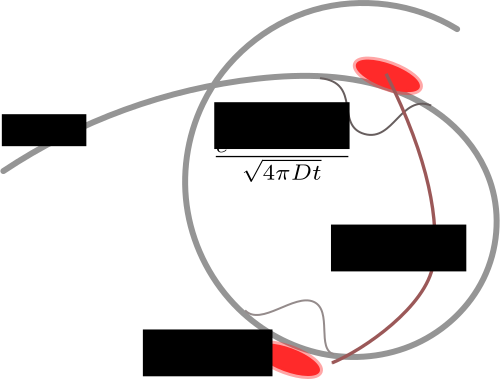
\includegraphics[width=0.7\textwidth]{TF_search.pdf}
	\caption{Illustration of combined 1D/3D search.}
	\label{fig:TF_search}
\end{figure}

\subsection*{Why is there an optimum?}
One dimensional diffusion alone would be extremely inefficient since it takes very long time to scan the entire genome due to the square-root scaling of the distance covered.
Very short $\tau_{1D}$, on the other hand, corresponds to very limited scanning of bases and in the limit of $\tau_{1D}\to 0$ corresponds to pure 3D search.
Hence it is plausible that an optimum should exist.


% accuracy
 %!TEX root = main.tex
\chapter{Discrimination and fidelity}

Many biochemical reactions happen at extreme fidelity: DNA replication in some organisms makes fewer than one mistake in $10^{10}$ bases copied.
Mutation rates vary greatly across organisms: the smaller the genome, the higher the mutation rate.
This anti-correlation is shown in schematically in Fig.~\ref{fig:mutation_rates}.
This fidelity relies on energetic discrimination of the correct and wrong base pairing.
The difference in interaction energies of the correct (Watson-Crick) and non-basepairing configuration, however, is only a few kT.
The fact that extremely high accuracies can be achieved is therefore remarkable.

\begin{figure}[tb]
	\centering
	\includegraphics[width=\textwidth]{figures/mutation_rates.jpg}
	\caption{Mutation rates of various organisms vs their genome size.}
	\label{fig:mutation_rates}
\end{figure}

Why should we expect such an anti-correlation?
The probability that that the entire genome of length $L$ is copied faithfully is given by $\exp(-L\mu)$.
Hence as soon as the mutation rate is much larger than the inverse genome size, almost every new genome will contain mutations resulting in a gradual loss of functional sequence (a process known as Muller's ratchet).
If being accurate is costly in terms of energy amd/or time, you'd expect organisms to adjust fidelity to be just ``good enough''. Hence the scaling behavior of fidelity with genome length is plausible.

However, it is not at all a trivial question how high fidelity can be achieved given the small free energy differences associated with nucleotide mis-incorporation.
It was \citep{hopfield_kinetic_1974} and \citep{ninio_kinetic_1975} who first discussed mechanisms on how to achieve high fidelity in biochemical processes.
Fidelity is not only important in DNA replication, but also in translation, tRNA charging and signaling processes.

\section{Energies of discrimination}
Consider the following simple set of reactions
\begin{equation}
C + E \leftrightarrow CE \rightarrow \mathrm{correct}
\end{equation}
\begin{equation}
D + E \leftrightarrow DE \rightarrow \mathrm{wrong}
\end{equation}
The transition states CE and DE are populated according to the equilibrium constant of these reactions $K_C =k_C'/k_C$ and $K_D = k_D'/k_D$ where $k'_C$  and $k'_D$ are the on-rates and $k_C$, $k_D$ are the off-rates.
We assume that the product formation happens at the same rate $W$ for both the correct and incorrect transition state.
In other words, the discrimination between the wrong and the correct state happens in the formation of the transition state.
This is a sensible assumption in cases like polymerization reactions which can occur as long as the two entities are in place.
Furthermore, it is reasonable to assume that the on-rates $k_C'$ and $k_D'$ are similar since they are likely limited by diffusion.
The off-rates, on the other hand, are strongly dependent on the correct substrate match and this is where discrimination comes from.
Assuming that both on-rates are $k = k_C' = k_D'$, we can express the rate at which each product is formed as
\begin{equation}
W[Cc] = W\frac{k[C]}{k_C+W}
\end{equation}
\begin{equation}
W[Dc] = W\frac{k[D]}{k_D+W}
\end{equation}
and hence the ratio of correct to wrong product is
\begin{equation}
\frac{\mathrm{correct}}{\mathrm{wrong}} = \frac{[C]}{[D]}\frac{k_D+W}{k_C + W} \rightarrow \frac{[C]}{[D]}\frac{k_D}{k_C} =  \frac{[C]}{[D]}e^{-\Delta G/kT}
\end{equation}
Here the last two expressions assumed that the product formation rate $W$ is much smaller than the off-rates of the transition state.
The very last equality expressed the off-rate dependence in terms of the difference in free energy of the transition states and thereby defines the {\bf energy of discrimination}.
Hence in any off-rate dominated discrimination, the differences in free energy put an upper bound on the accuracy of the process.
However, the binding energy differences of incorrect nucleotide reactions are on the order of a few kT and while accuracy of DNA replication would seem to require energies of discrimination on the order of 20kT.
This conundrum is what kinetic proofreading resolves in an elegant way.

\section{Irreversible intermediate states and kinetic proof reading}
Kinetic proof reading requires additional steps in the pathway to final product, but at least one of these steps needs to be coupled to an additional energy consuming reaction that makes the pathway irreversible.
The need for such an additional step is seen as follows: A reaction that proceeds via two intermediate states $XE$ and $XE'$ can effectively be compressed into one
\begin{equation}
X + E \leftrightarrow XE \leftrightarrow  XE' \rightarrow \mathrm{product}
\end{equation}
\begin{equation}
X + c \leftrightarrow  XE' \rightarrow \mathrm{product}
\end{equation}
or put otherwise the second intermediate state is in equilibrium with the same discriminatory ratio as before.

If, however, the transition from $XE$ to $XE' $ is coupled to an irreversible reaction while $XE'$ can still decay into $X+E$, higher accuracy can be attained.
In this case, the state $XE'$ can only be reached via $XE$ which is already selected for the correct product by a factor $e^{-\Delta G/kT}$.
If the rates of decay of $XE'$ for C and D are again different by a factor $e^{-\Delta G/kT}$, the overall accurary of the process can be as high as $e^{-2\Delta G/kT}$.

The accuracy of a process can be increased exponentially by adding more and more intermediate states.

\subsection*{Interpretation of proof-reading as a delay}
The addition of an irreversible step essentially changes the distribution of times the product spends in the transition state.
While being in the transition state, the correct pair decays as $e^{-k_Ct}$ and the wrong product as $e^{-k_Dt}$ such that the ratio behaves as $e^{-(k_C-k_D)t}$.
In a one step reaction, the distribution of residence times in the transition state has a peak at $t=0$ and decays exponentially. In a two-step reaction, this distributions has a peak away from zero.
This can be seen as follows.
Consider the a transition state $XE$ the moment it is formed. The probability $p(t)$ of still being intact is given by
\begin{equation}
\frac{dp}{dt} = - (k_X + W)p(t) \quad \Rightarrow\quad p(t) = e^{-(k_X+W)t}
\end{equation}
where $W$ is the rate at which the second intermediate is formed.
The probability $q(t)$ of being in the second intermediate is then
\begin{equation}
\frac{dq}{dt} = Wp(t) - Vq(t) = We^{-(k_X+W)t} - Vq(t)
\end{equation}
The latter has the solution
\begin{equation}
q(t) = We^{-Vt}\int_0^t e^{(V-W-k_X)t'} dt' = \frac{We^{-Vt}}{W+k_X-V}\left[1-e^{-(W+k_X - V)t}\right]
\end{equation}
While in a single step reaction the product starts being formed immediately, product formation starts gradually in a two step reaction.
This delay give the wrong intermediate complexes more time to break up and hence better discrimination.


\bibliography{bib}
\end{document}



% chromatin organization
\input{chapter_4}

% gene regulation in space and time
\input{chapter_5}



